\documentclass{beamer}
\usepackage{multimedia}
\usepackage{hyperref}
\usetheme{Madrid}
\title[Elaborato PPM]{\large Elaborato esame Progettazione e Produzione Multimediale}
\author[Francesco Bettazzi, Francesco Fantechi]{Francesco Bettazzi \and Francesco Fantechi}
\date[UNIFI 2020-2021]{A.A. 2020-2021}

\institute[]{

\begin{figure}[!h]
\centering

\includegraphics[width=2.5cm, height=2.5cm]{"Immagini/LogoUnifi.PNG"}
\end{figure}

%\begin{center}
UNIVERSITA' DEGLI STUDI DI FIRENZE \\
Facolta di Ingegneria \\
Corso di Laurea in Ingegneria Informatica
%\end{center}
}

\begin{document}

\frame{\titlepage}

\begin{frame}
\frametitle{Etch\&Post}
\begin{columns}
\column{0.5\textwidth}
\begin{itemize} 
\item <1-> Descrizione del sito
\begin{itemize}
 \item <2-> Visualizzare monumenti nelle vicinanze dell'utente su una mappa
 \item <3-> Postare foto dei punti di interesse in forma anonima
 \item <4-> Lasciare dei graffiti o dei messaggi su di esse
\end{itemize}
\item <5-> All'apertura del sito
\begin{itemize}
	\item <6-> Mappa geografica
	\item <7-> Popup rosso che indica la posizione realtime dell'utente
	\item <8-> Cluster che raggruppano i popup che rappresentano i POI nelle vicinanze o dove sono state postate foto
\end{itemize}

\end{itemize} 
\column{0.5\textwidth}
\begin{itemize}
	\item[] <5-> 
		\begin{figure}[!h]
 			\centering
 			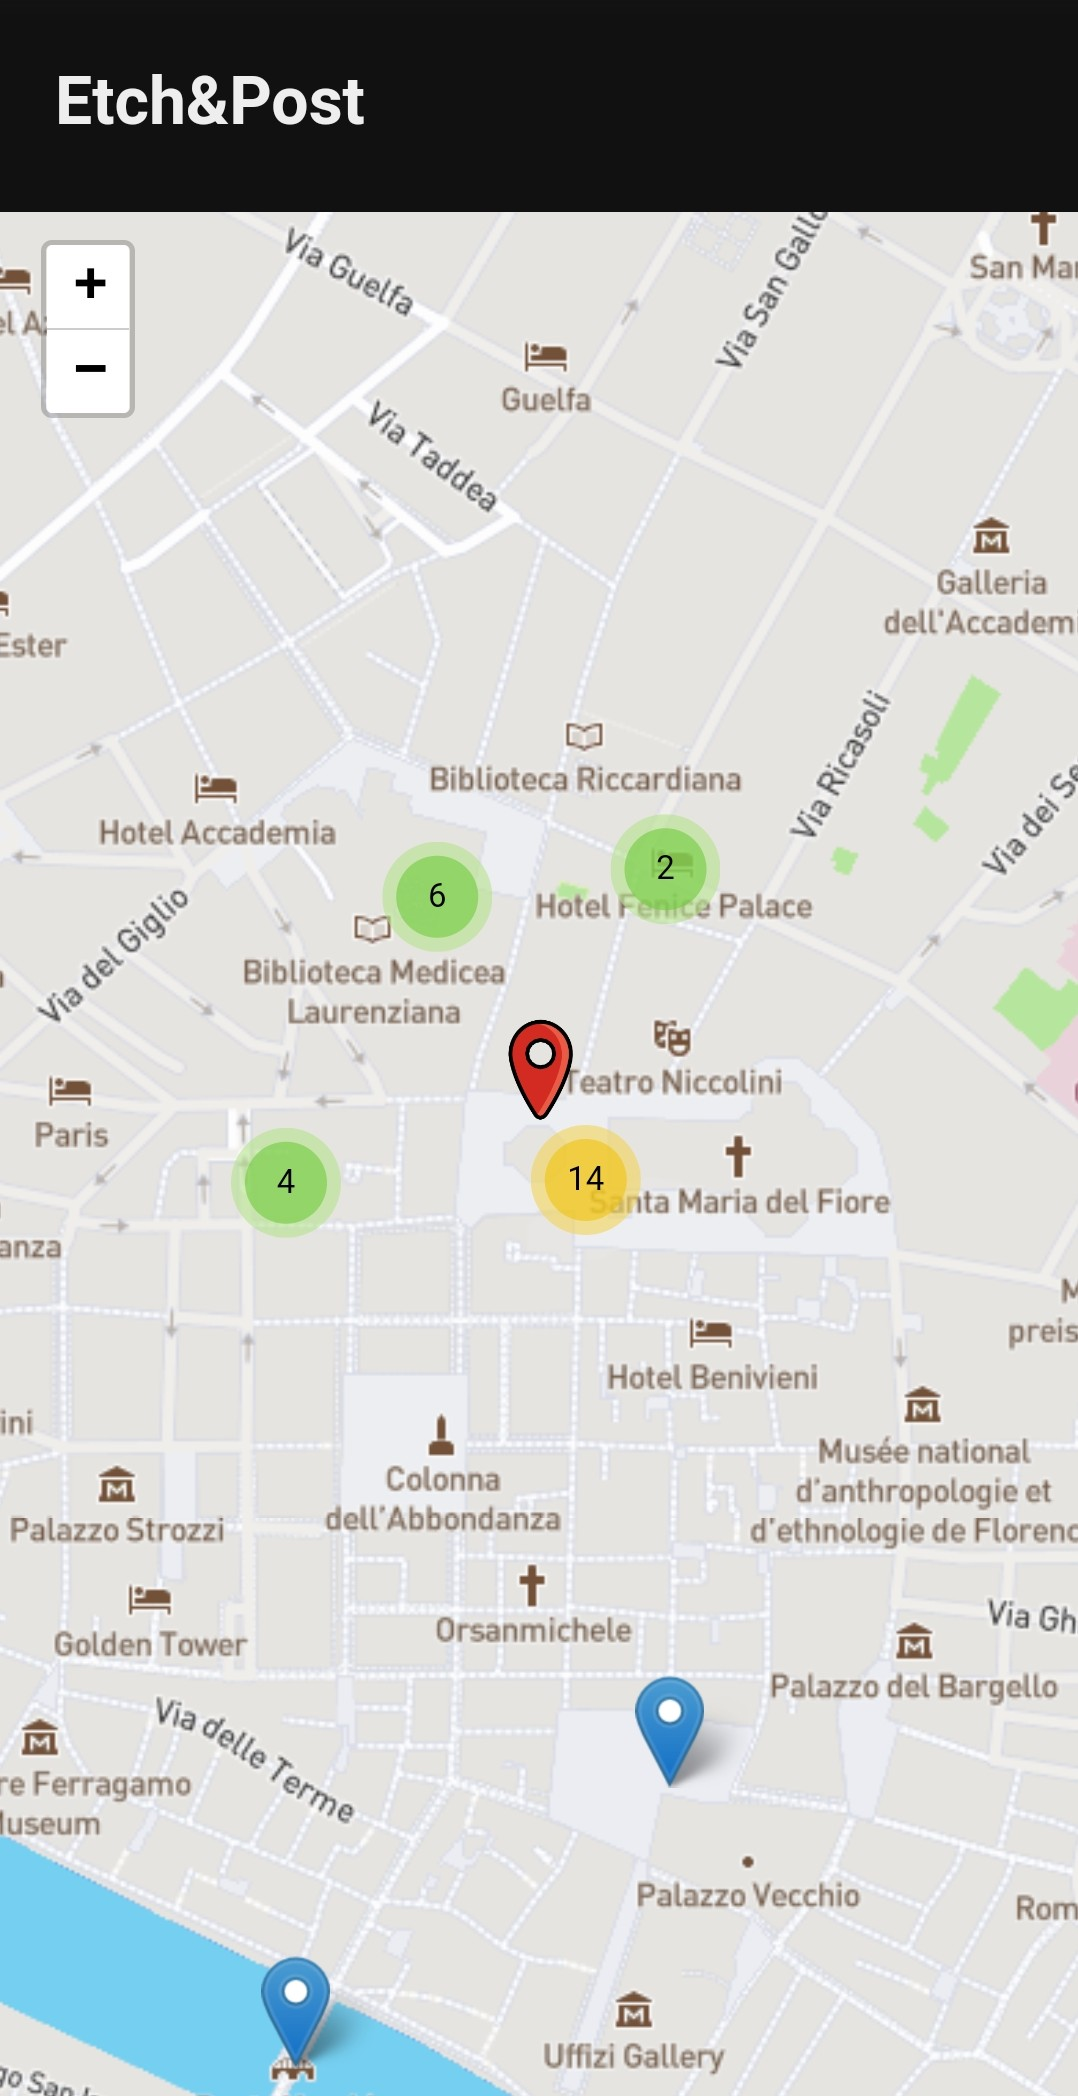
\includegraphics[scale=0.1]{"Immagini/Apertura.jpg"}
 		\end{figure}
\end{itemize}
\end{columns}
\end{frame}

\begin{frame}
\frametitle{Popup}
\begin{columns}
\column{0.5\textwidth}
\begin{itemize}
 \item <1-> Popup fotocamera se POI entro 200 metri dall'utente
 \item <2-> Popup galleria se POI pi\`u distante dall'utente e con delle foto postate
 \item <3-> Popup con fotocamera e galleria se POI entro 200 metri dall'utente e con foto postate
\end{itemize}

\column{0.5\textwidth}
\begin{itemize}
	\item[] <1|only@1> 
		\begin{figure}[!h]
 			\centering
 			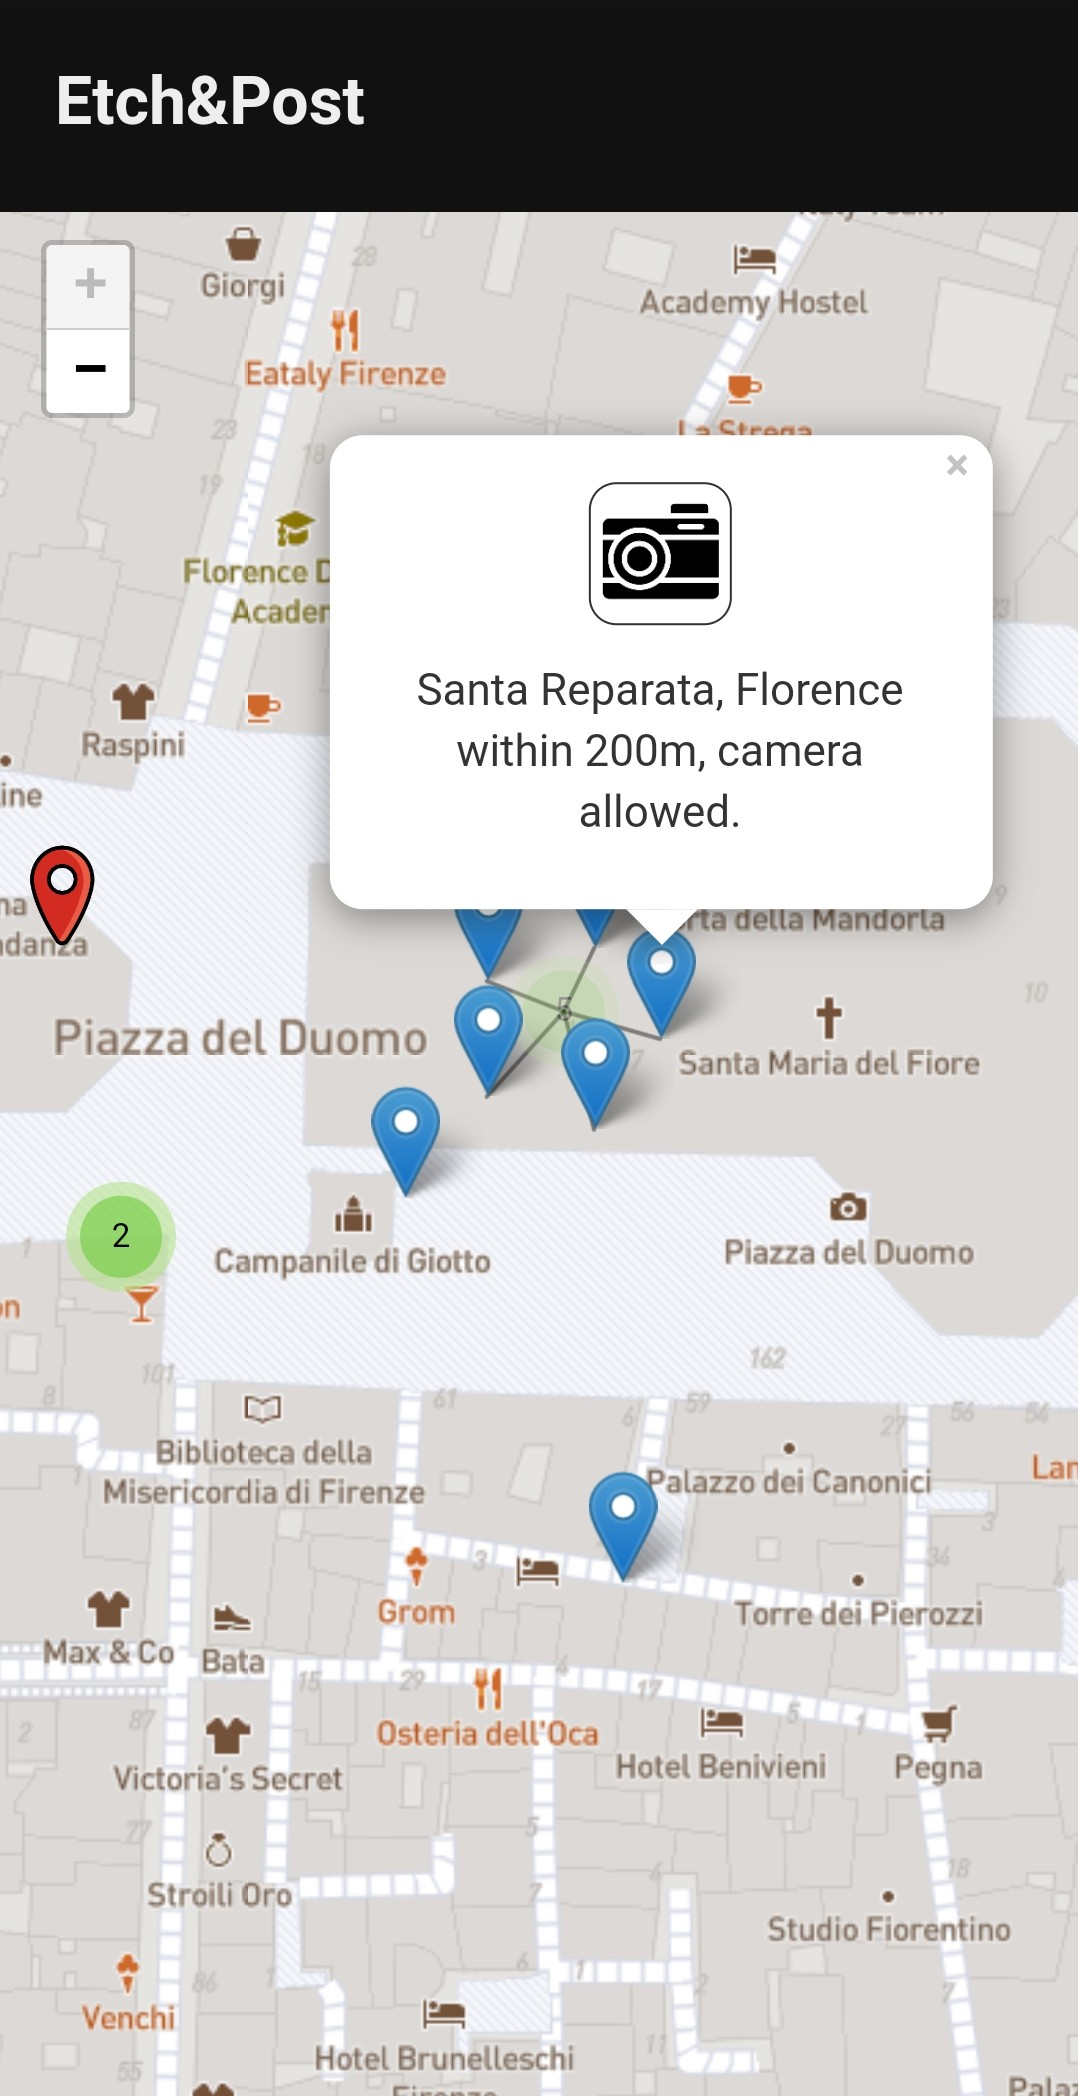
\includegraphics[scale=0.1]{"Immagini/camera.jpg"}
 		\end{figure}
 	\item[] <2|only@2> 
		\begin{figure}[!h]
 			\centering
 			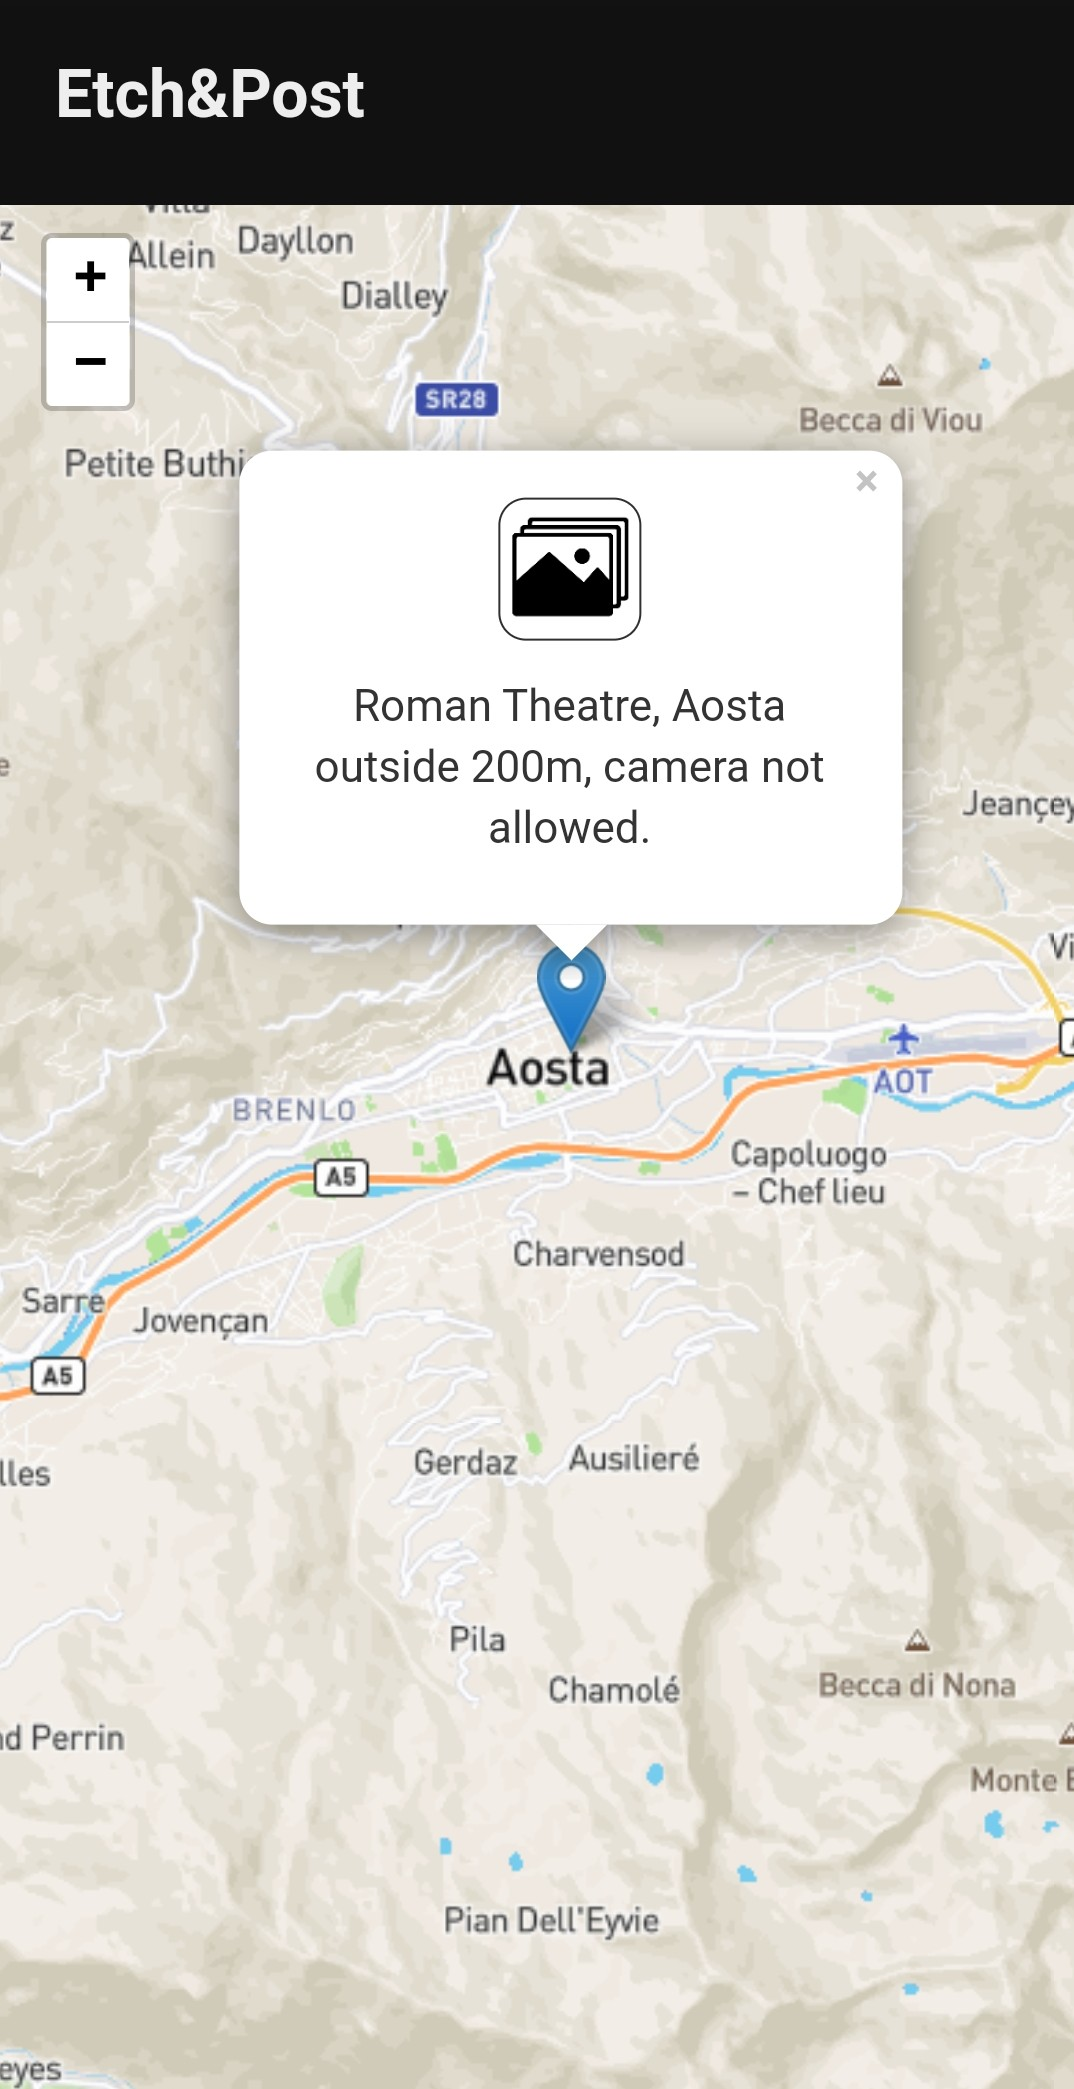
\includegraphics[scale=0.1]{"Immagini/galleria.jpg"}
 		\end{figure}
 	\item[] <3|only@3> 
		\begin{figure}[!h]
 			\centering
 			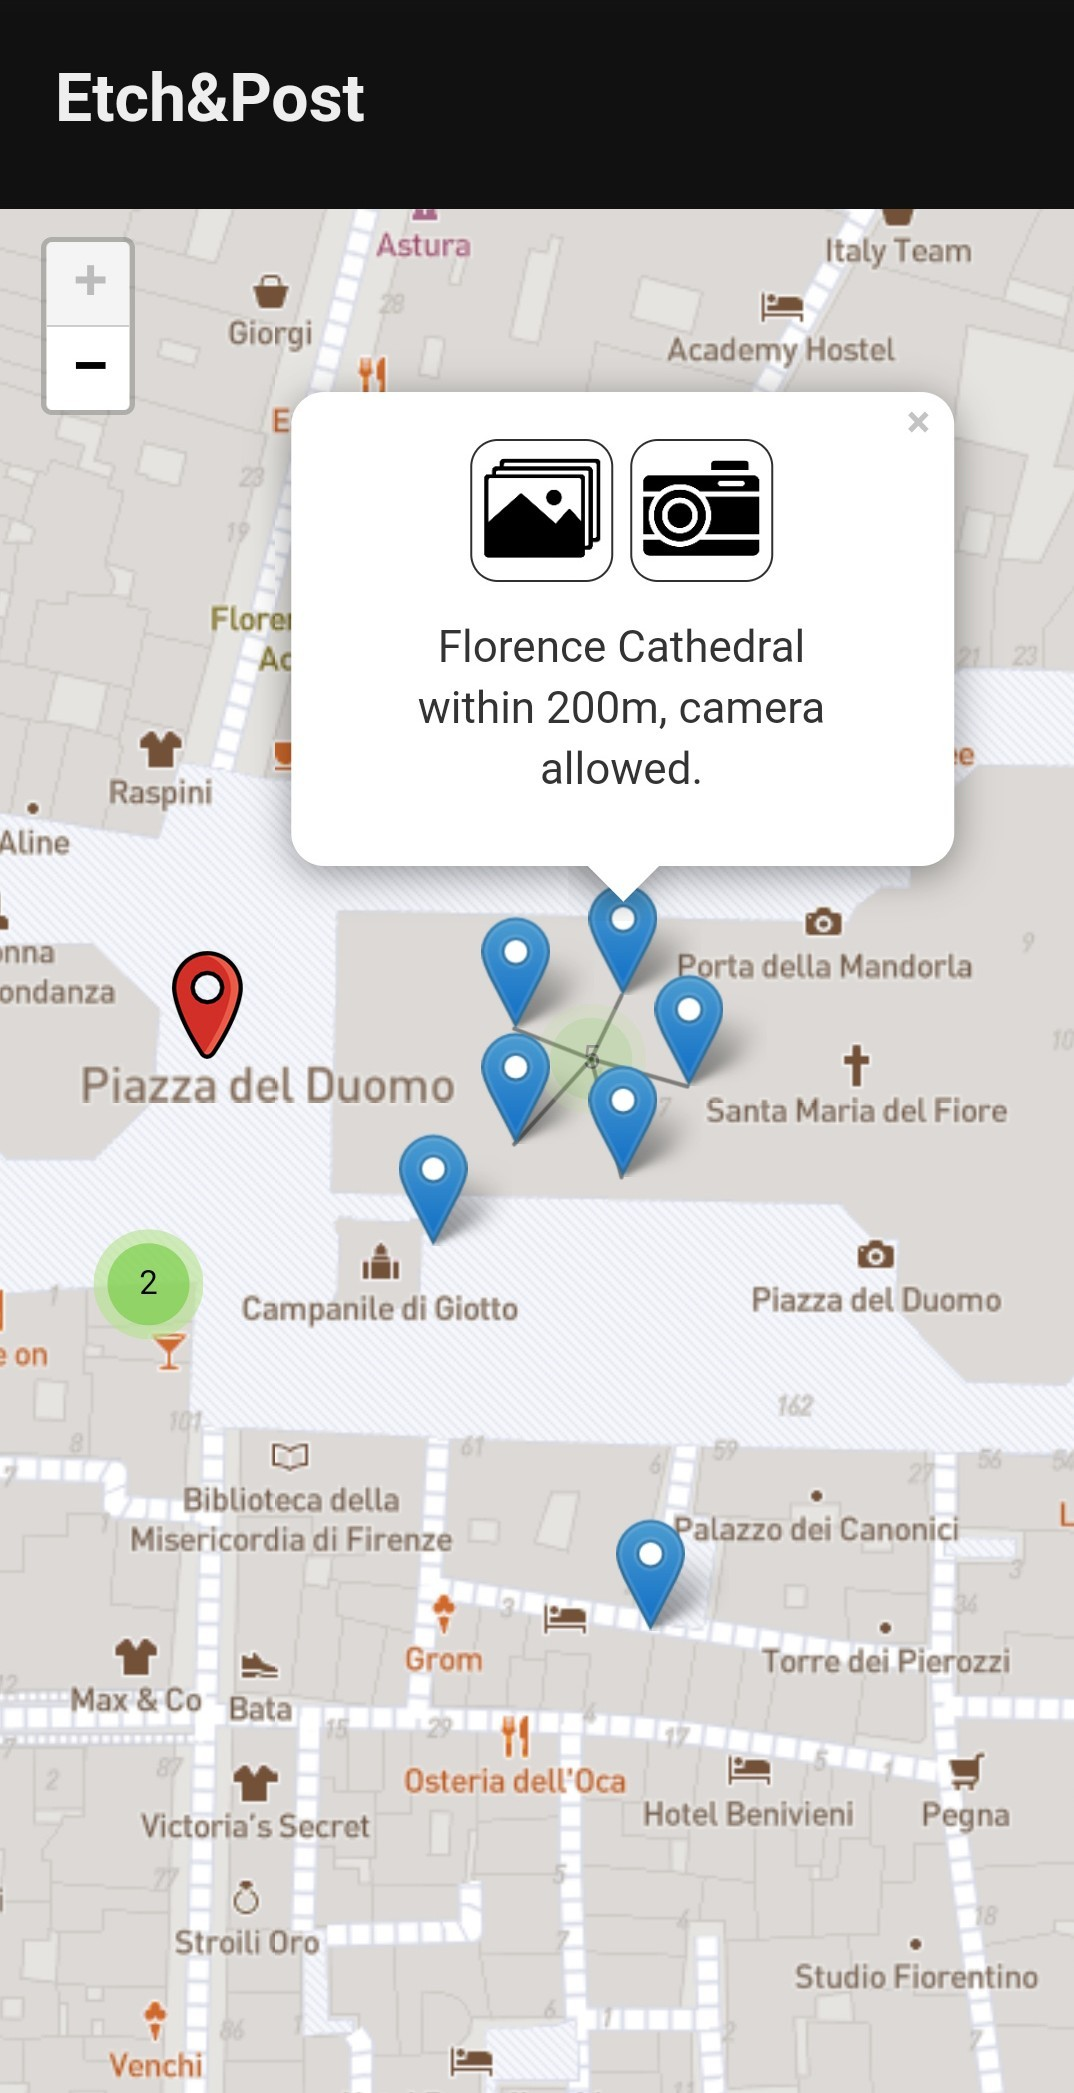
\includegraphics[scale=0.1]{"Immagini/double.jpg"}
 		\end{figure}
\end{itemize}
\end{columns}
\end{frame}


\begin{frame}
\frametitle{Fotocamera}
\begin{columns}
\column{0.5\textwidth}
\begin{itemize}
	\item <2-> Nome del POI a cui si vuole scattare una foto
 	\item <3-> Pulsante per tornare alla mappa e chiudere la fotocamera
 	\item <4-> Pulsante per fare lo switch da fotocamera anteriore a posteriore se il dispositivo lo supporta
 	\item <5-> Pulsante per scattare la foto e aprire l'editor
\end{itemize}


\column{0.5\textwidth}
\begin{itemize}
	\item[] <1|only@1> 
		\begin{figure}[!h]
 			\centering
 			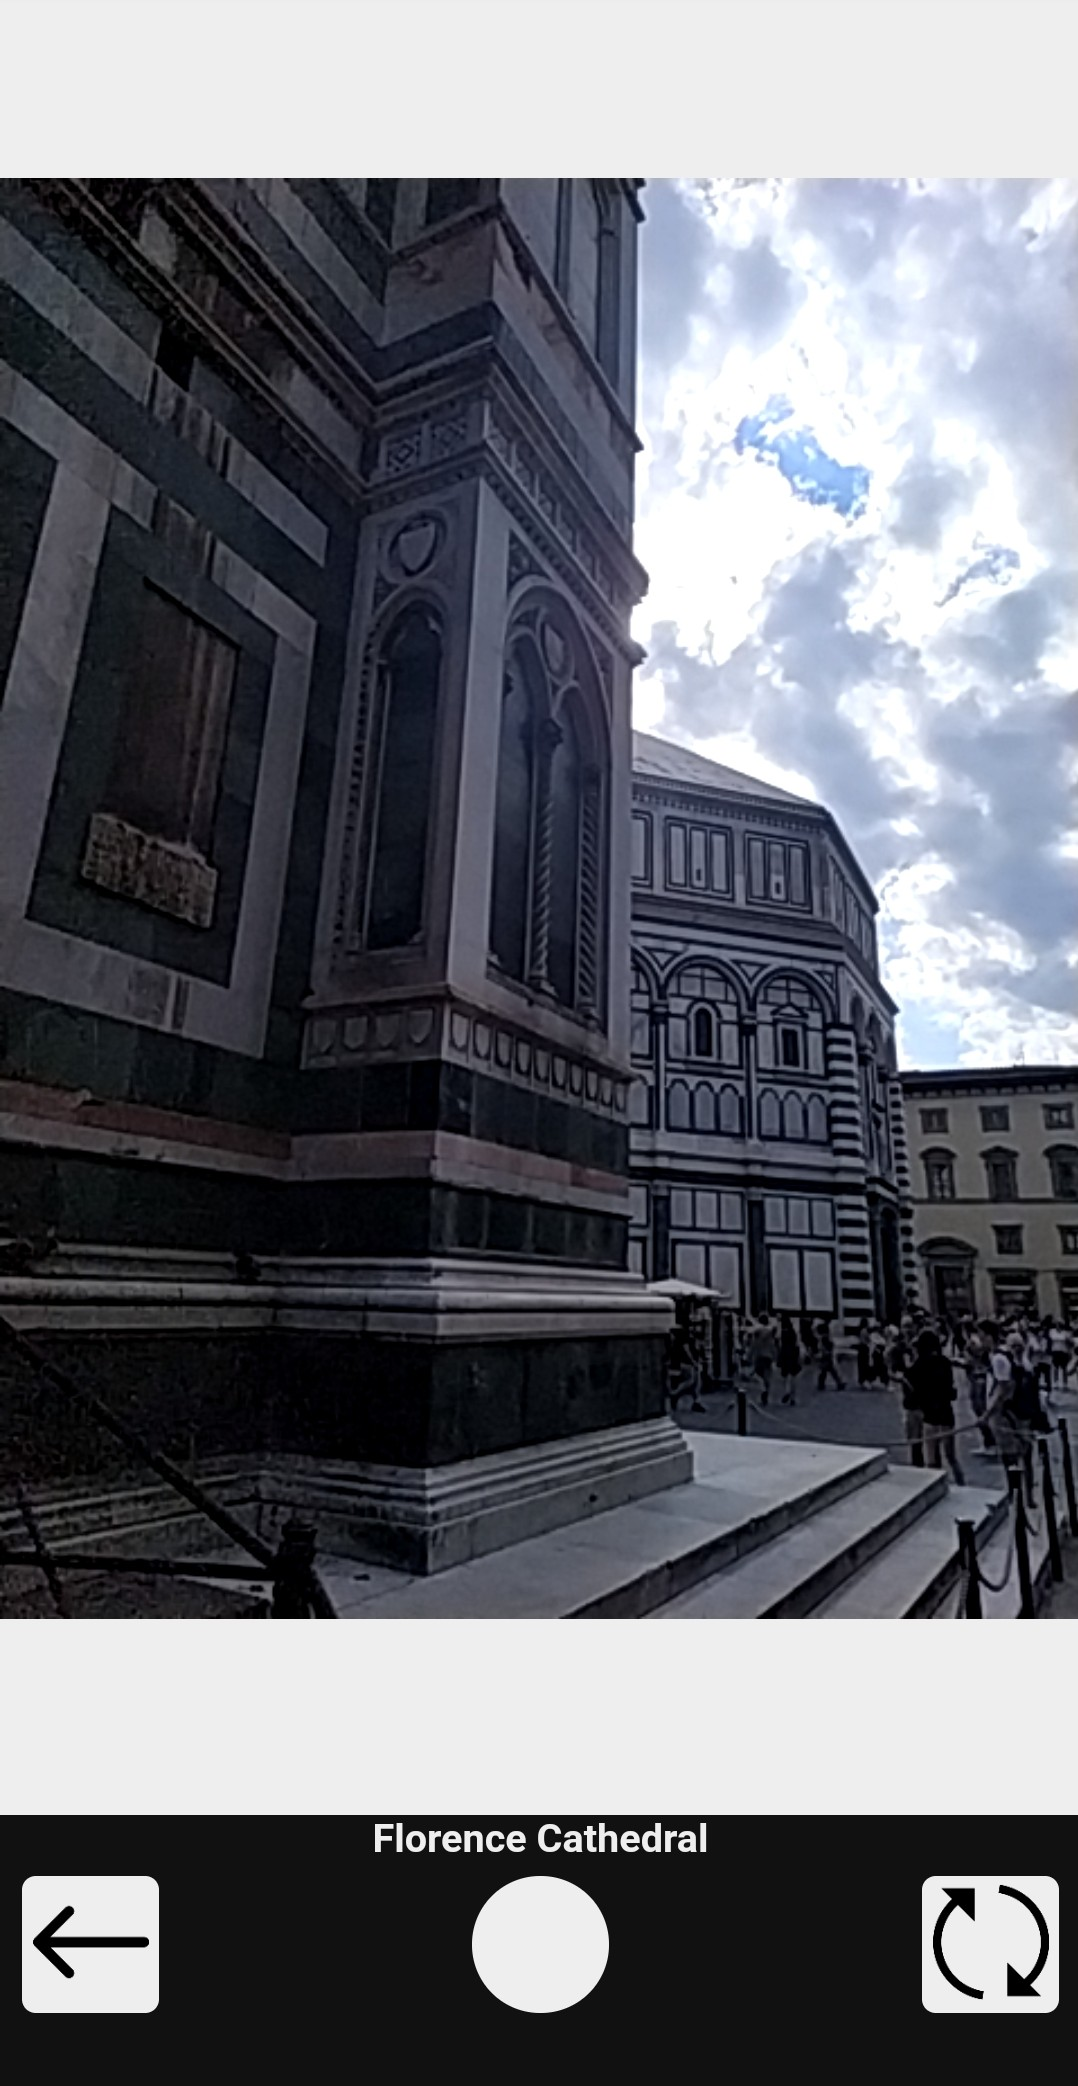
\includegraphics[scale=0.1]{"Immagini/open_camera.jpg"}
 		\end{figure}
 	\item[] <2|only@2> 
		\begin{figure}[!h]
 			\centering
 			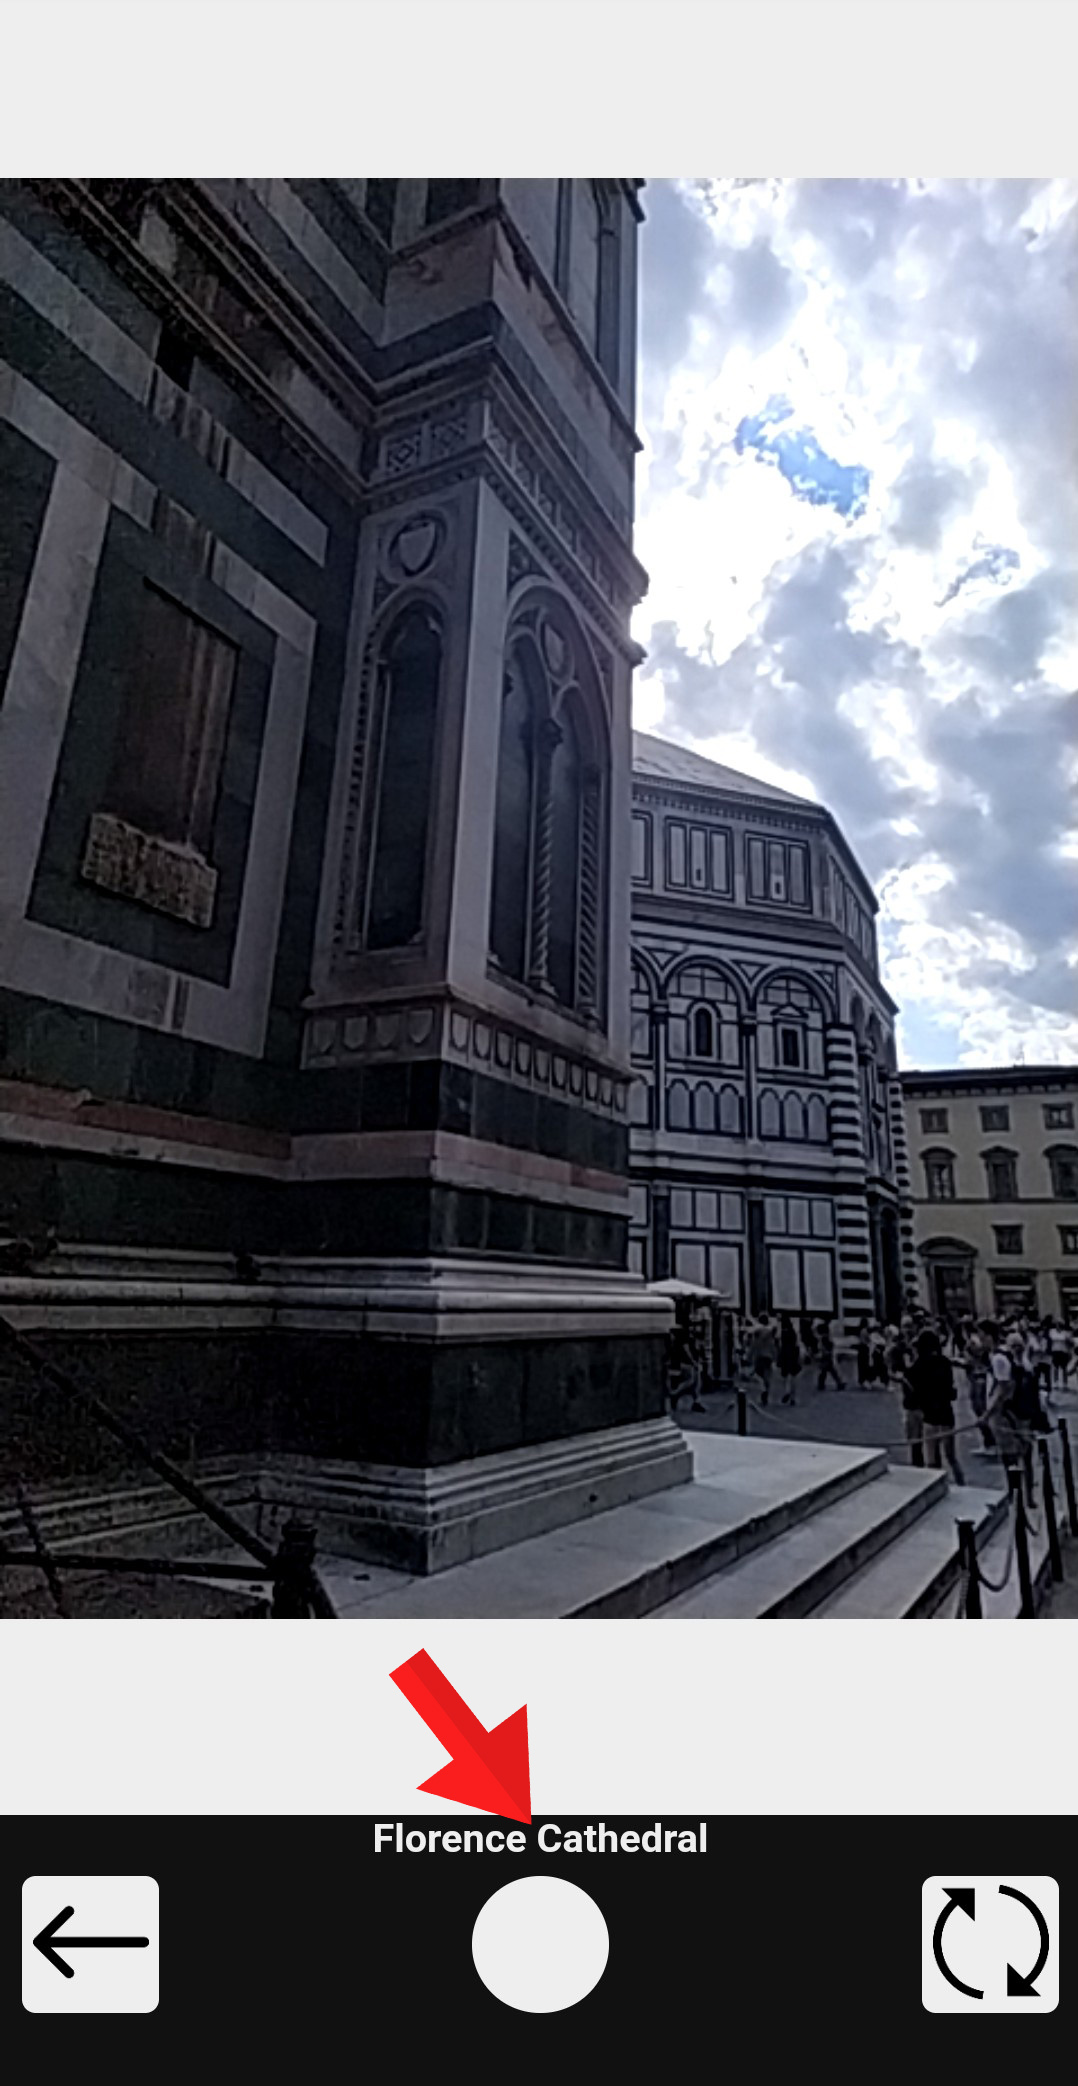
\includegraphics[scale=0.1]{"Immagini/open_camera1.jpg"}
 		\end{figure}
 	\item[] <3|only@3> 
		\begin{figure}[!h]
 			\centering
 			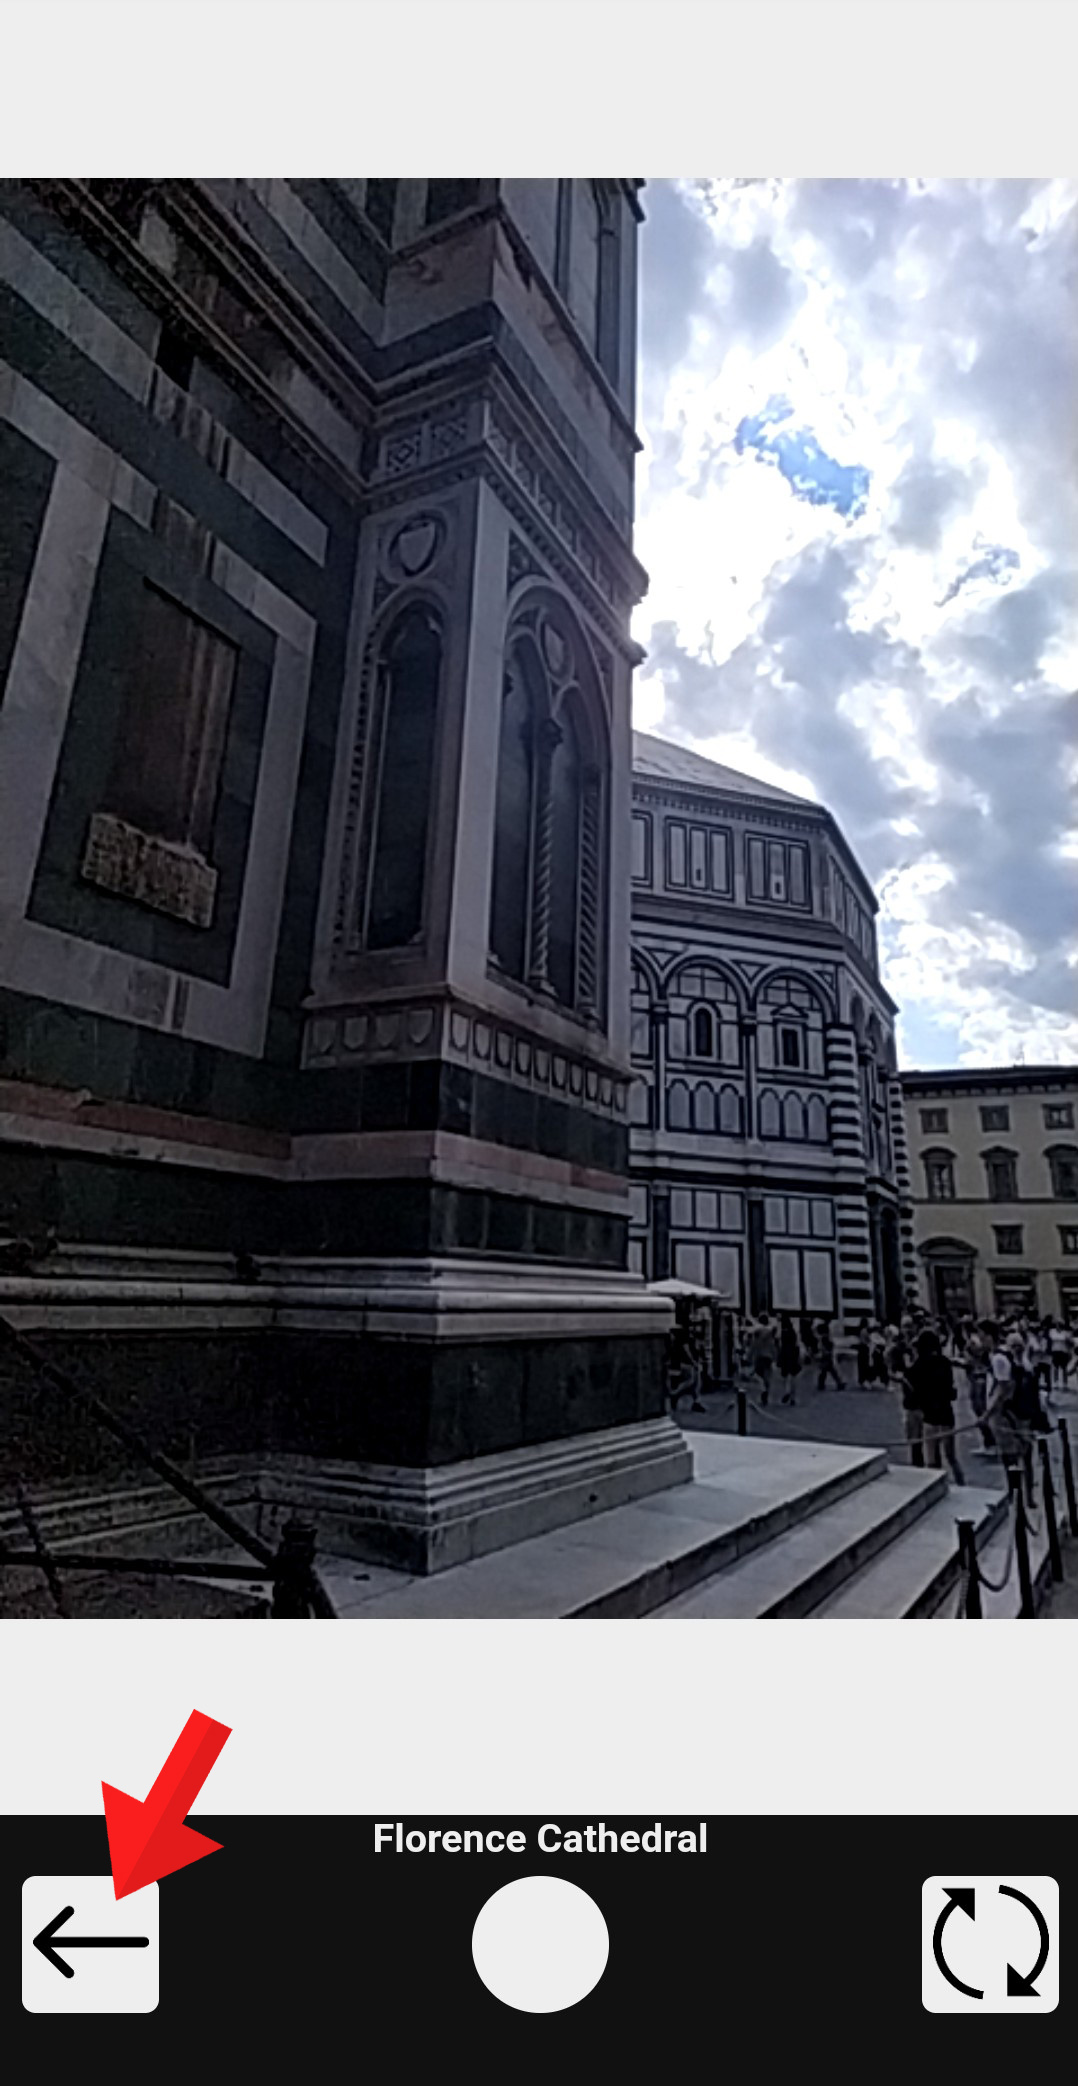
\includegraphics[scale=0.1]{"Immagini/open_camera2.jpg"}
 		\end{figure}
 	\item[] <4|only@4> 
		\begin{figure}[!h]
 			\centering
 			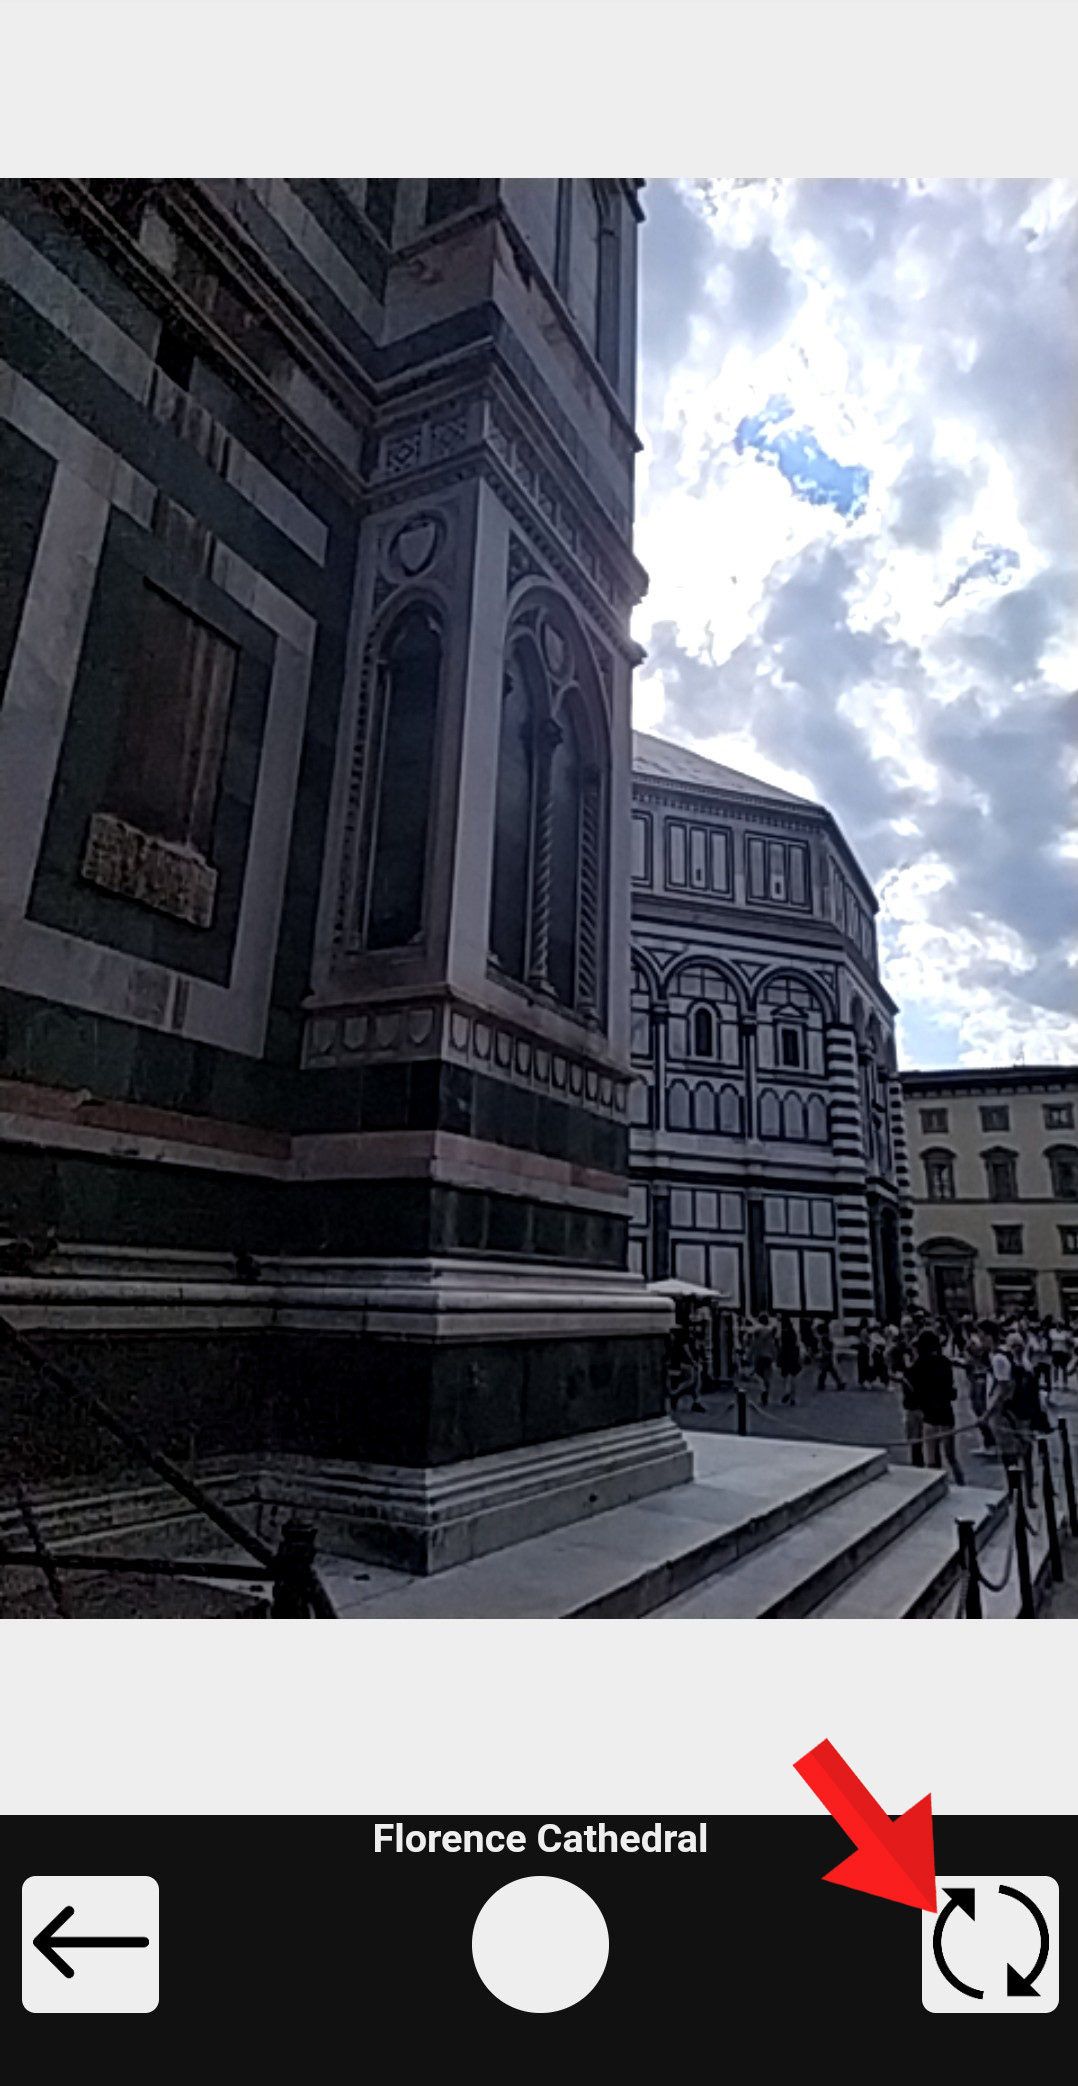
\includegraphics[scale=0.1]{"Immagini/open_camera3.jpg"}
 		\end{figure}
 	\item[] <5|only@5> 
		\begin{figure}[!h]
 			\centering
 			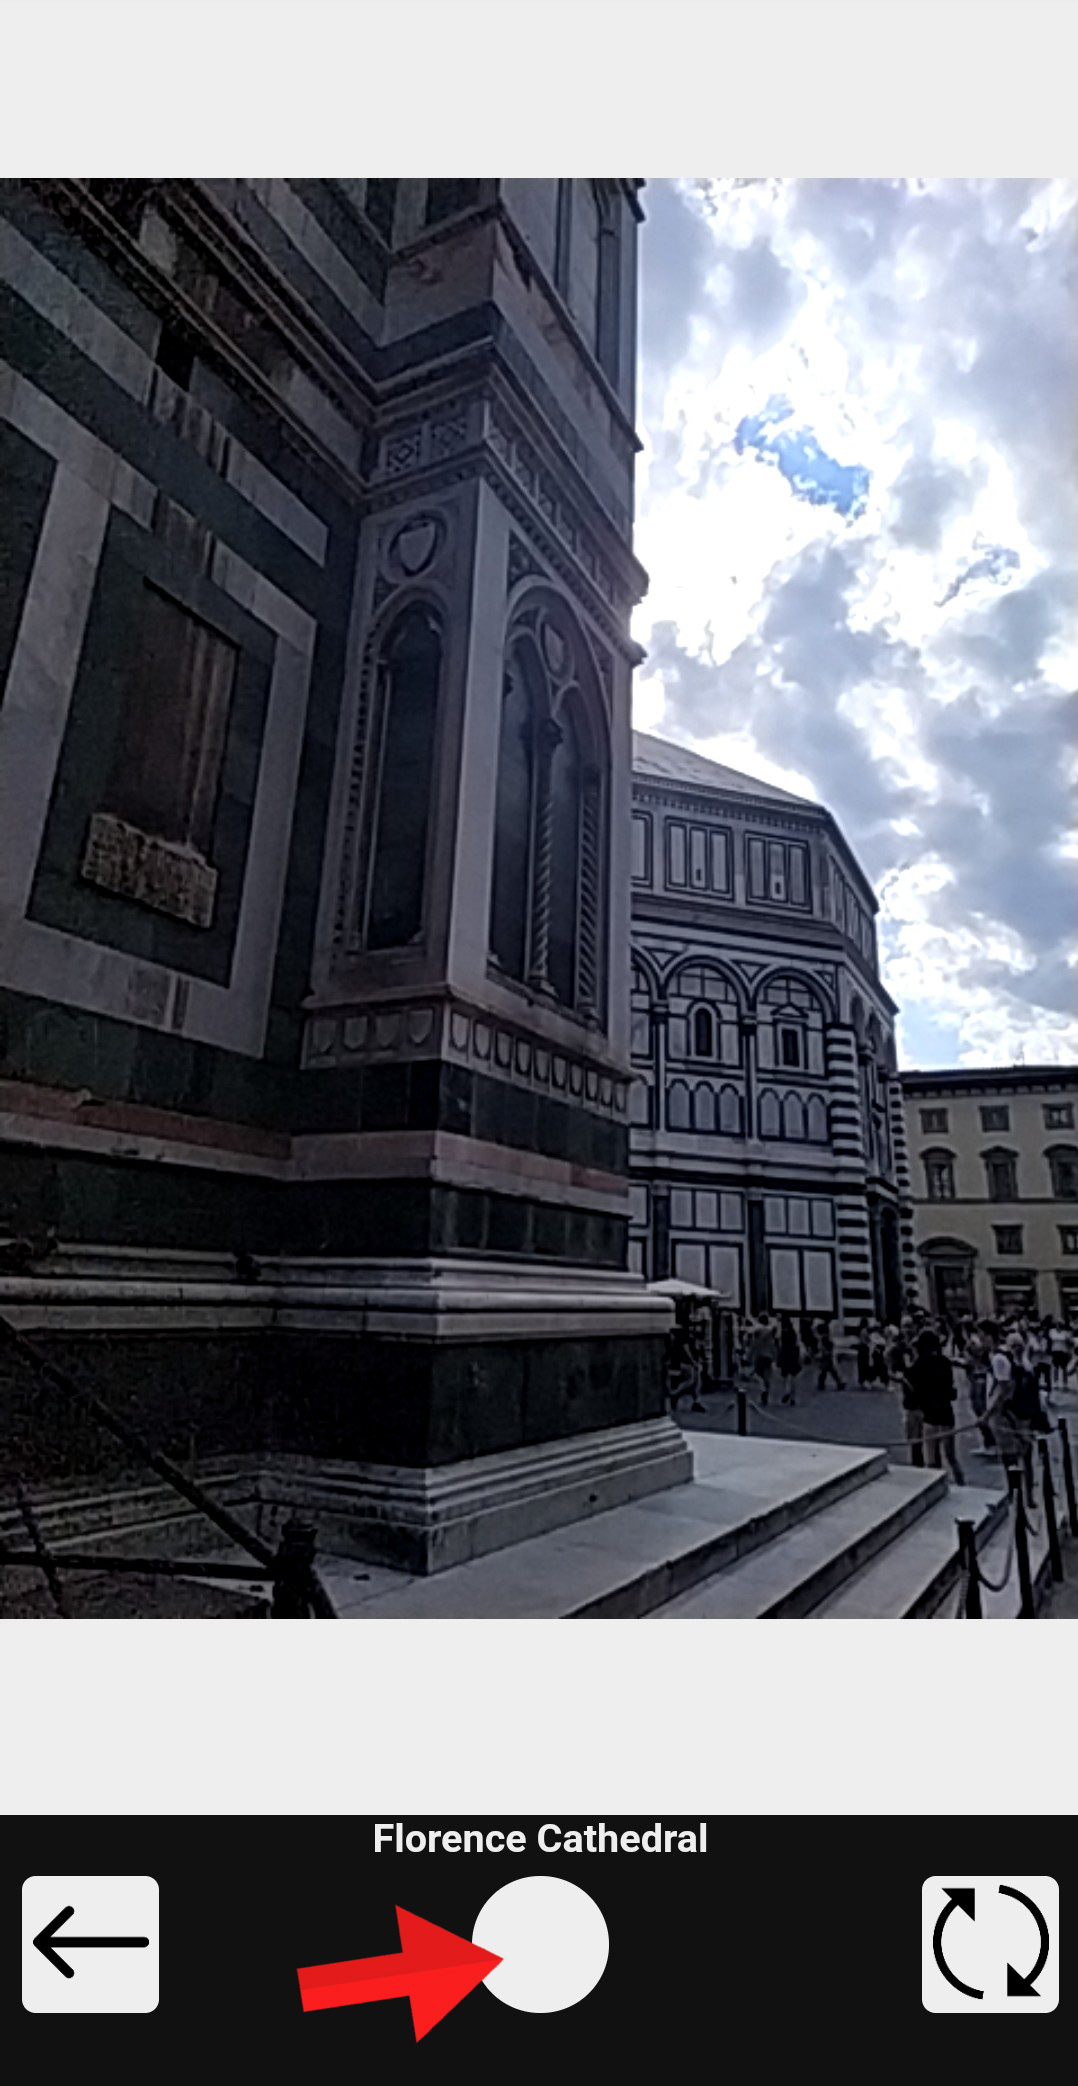
\includegraphics[scale=0.1]{"Immagini/open_camera4.jpg"}
 		\end{figure}
\end{itemize}
\end{columns}
\end{frame}

\begin{frame}
\frametitle{Editor}
\begin{columns}
\column{0.5\textwidth}
\begin{itemize}
 	\item <2-> Nome del POI a cui si \`e scattata la foto
 	\item <3-> Pulsante per scegliere il colore con cui disegnare sulla foto 
 	\item <5-> Pulsante per cancellare tutti i graffiti fatti sull'immagine
 	\item <6-> Pulsante per scartare la foto e tornare alla fotocamera
 	\item <7-> Pulsante per postare la foto con le modifiche fatte sul POI scelto
\end{itemize}


\column{0.5\textwidth}
\begin{itemize}
	\item[] <1|only@1> 
		\begin{figure}[!h]
 			\centering
 			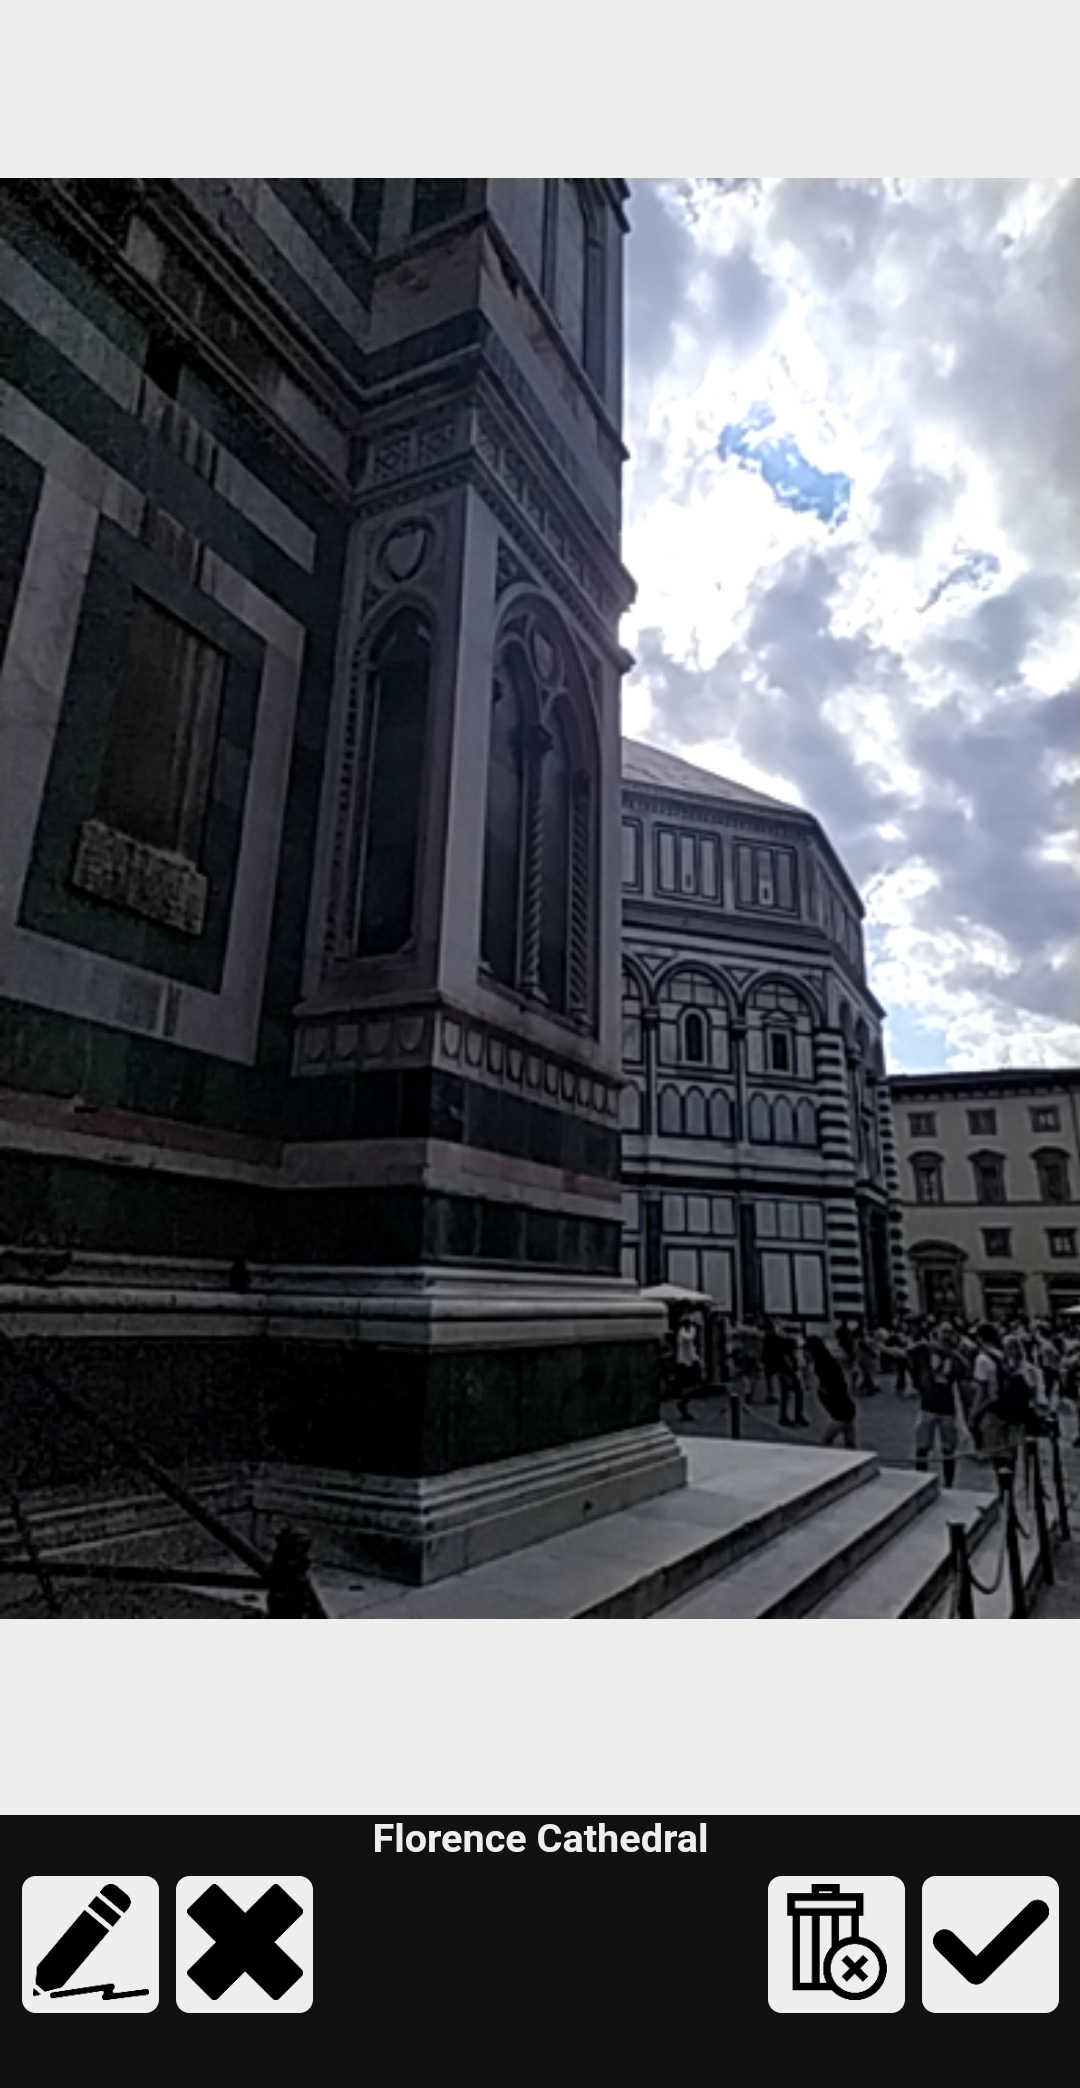
\includegraphics[scale=0.1]{"Immagini/editor0.jpg"}
 		\end{figure}
 	\item[] <2|only@2> 
		\begin{figure}[!h]
 			\centering
 			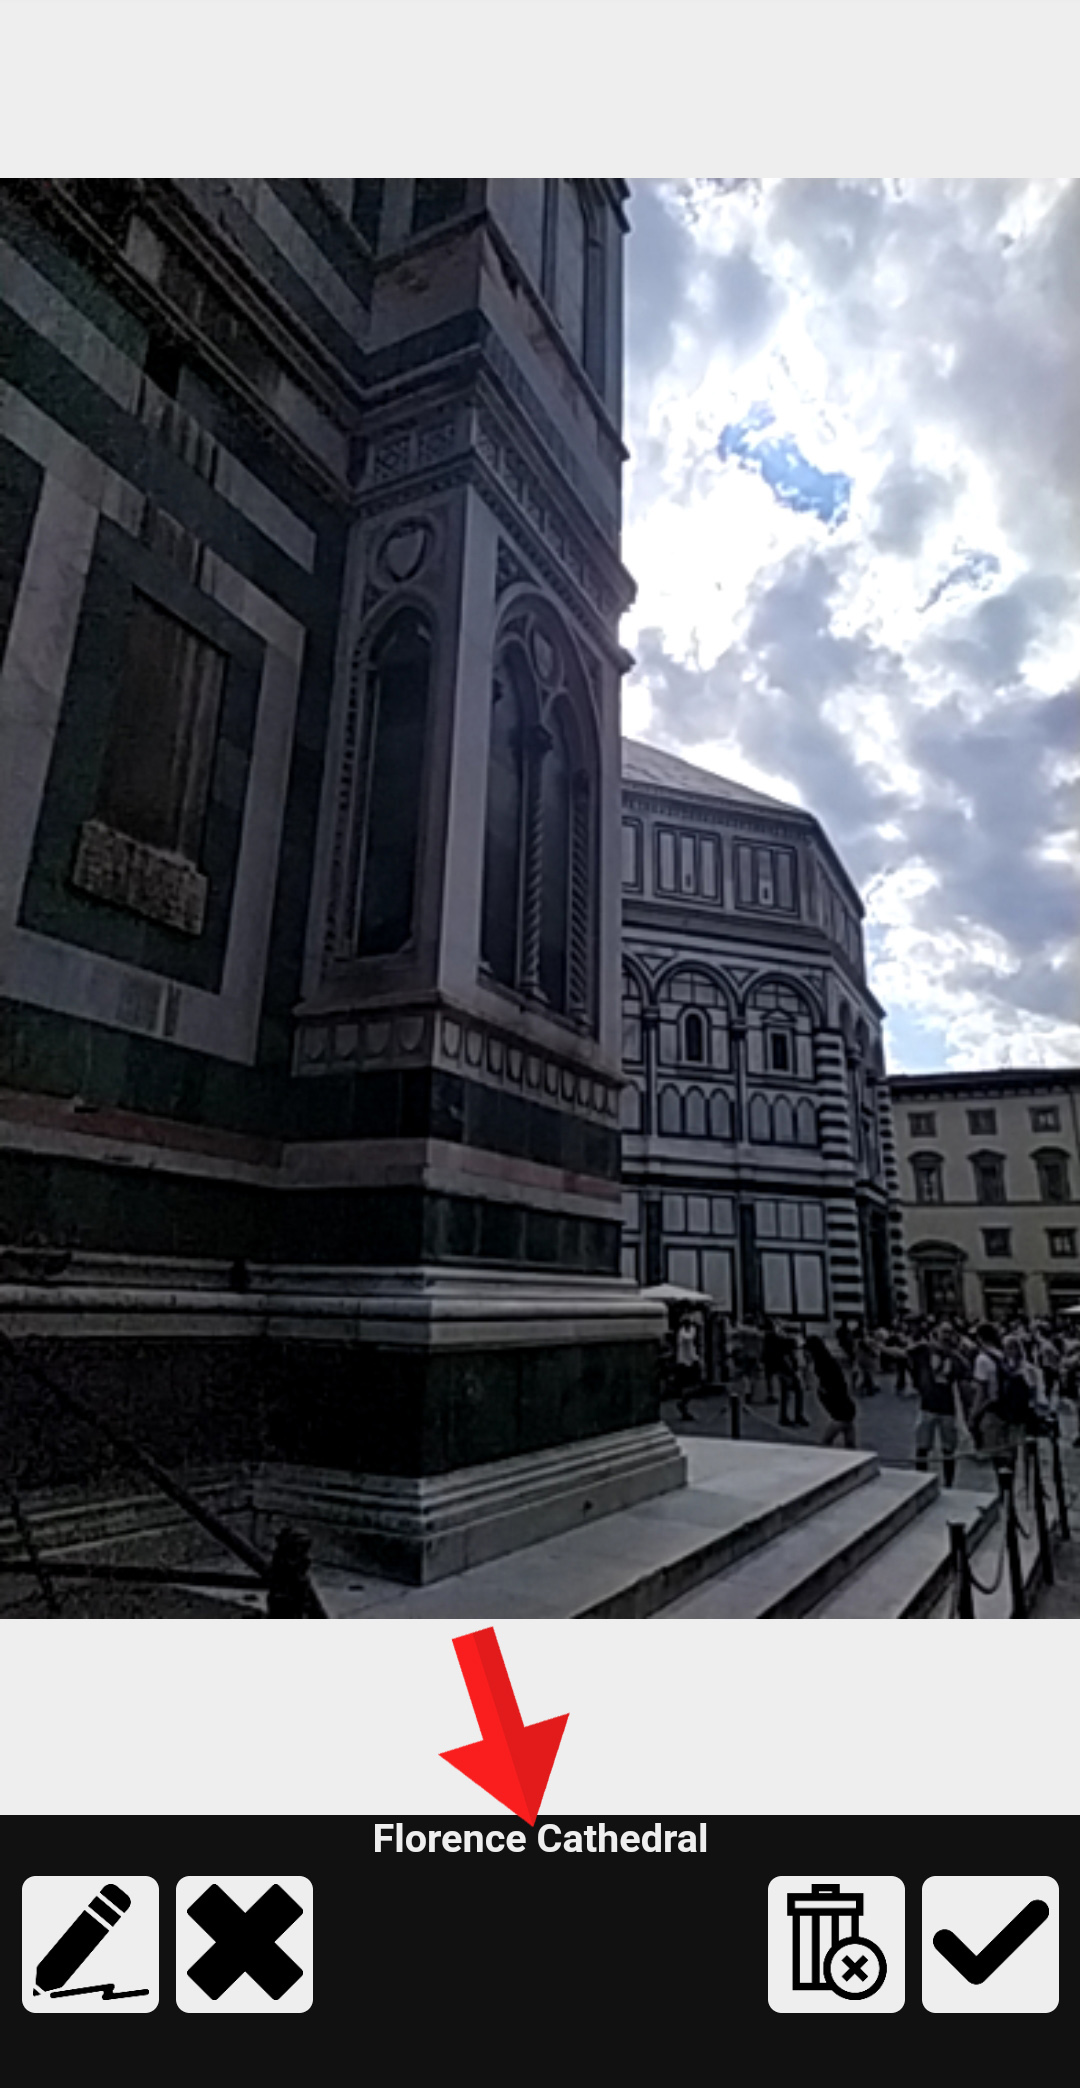
\includegraphics[scale=0.1]{"Immagini/editor4.jpg"}
 		\end{figure}
 	\item[] <3|only@3> 
		\begin{figure}[!h]
 			\centering
 			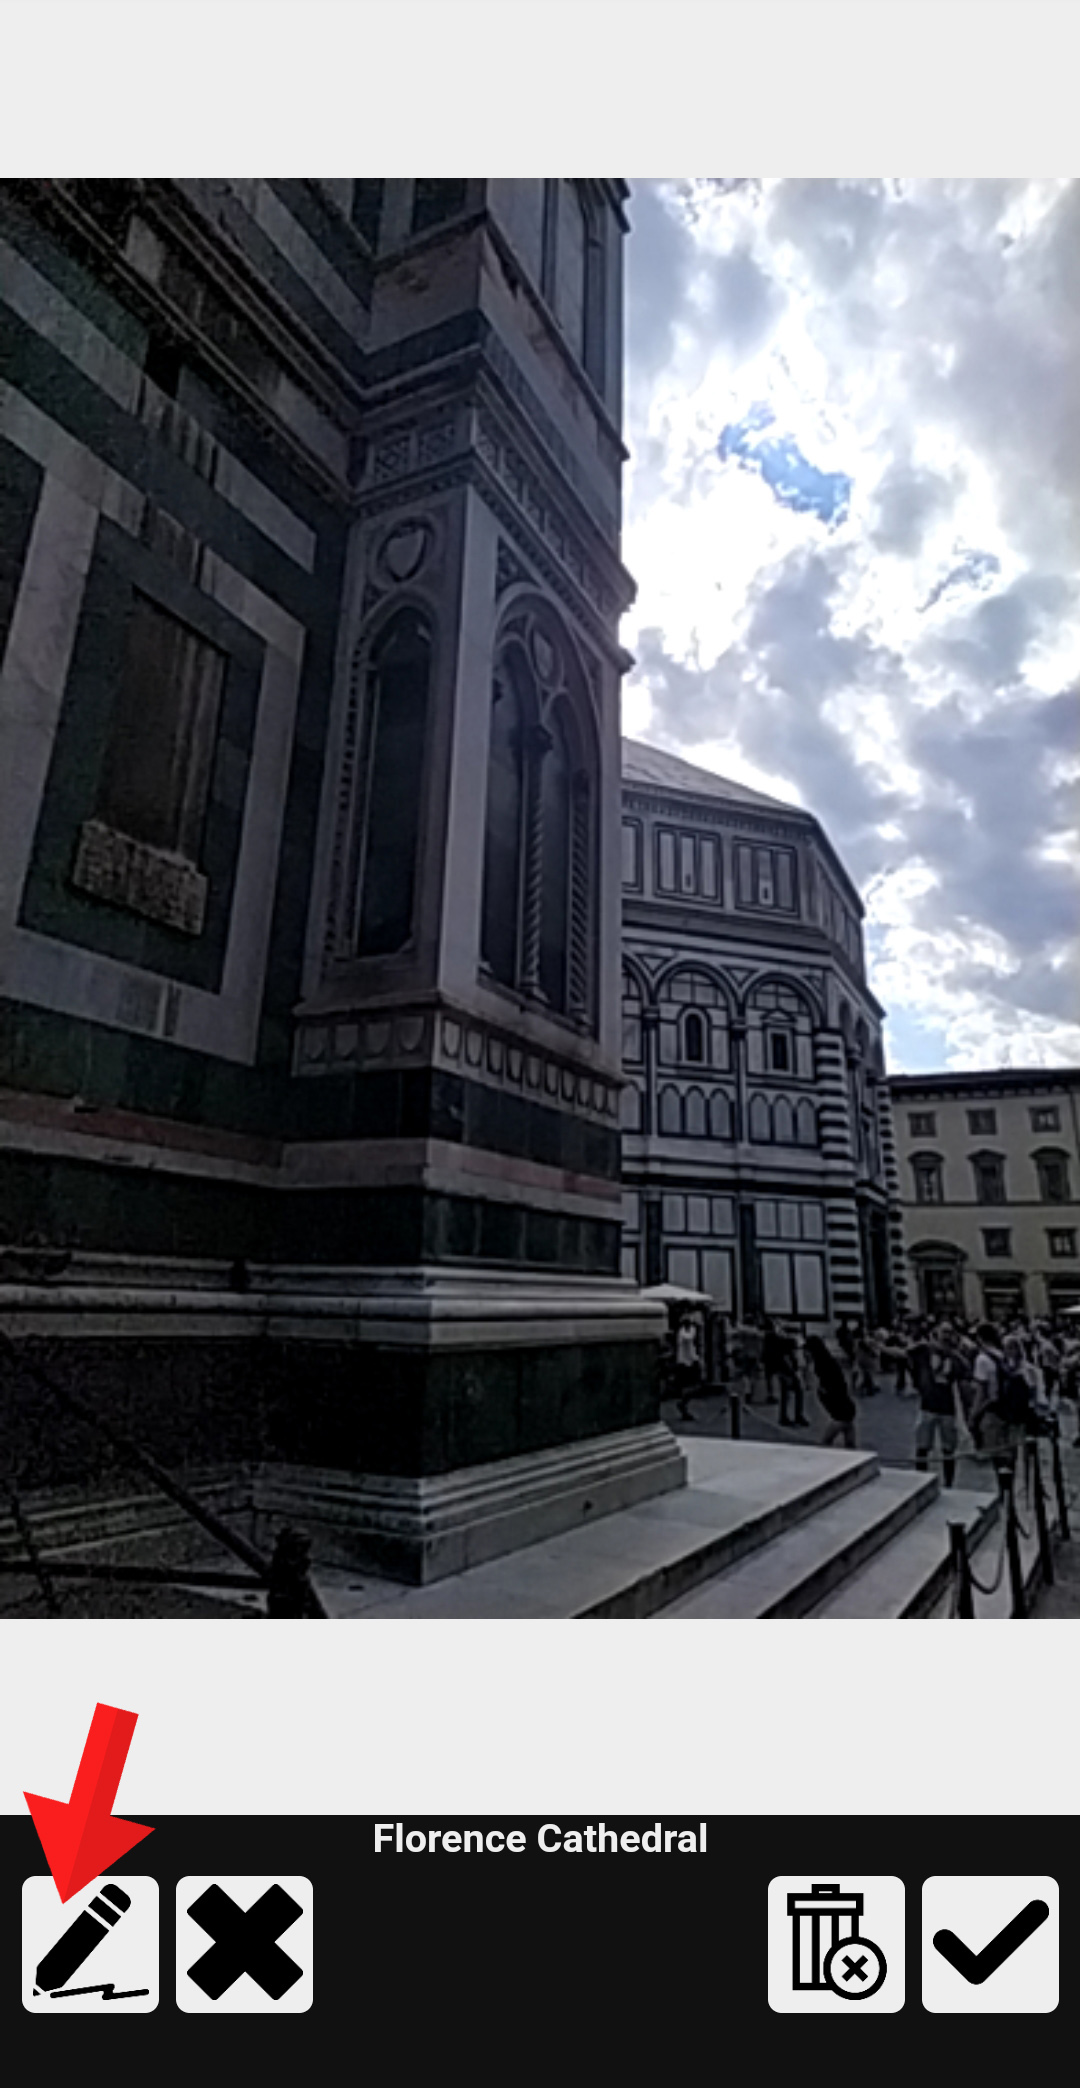
\includegraphics[scale=0.1]{"Immagini/editor2.jpg"}
 		\end{figure}
 	\item[] <4|only@4> 
		\begin{figure}[!h]
 			\centering
 			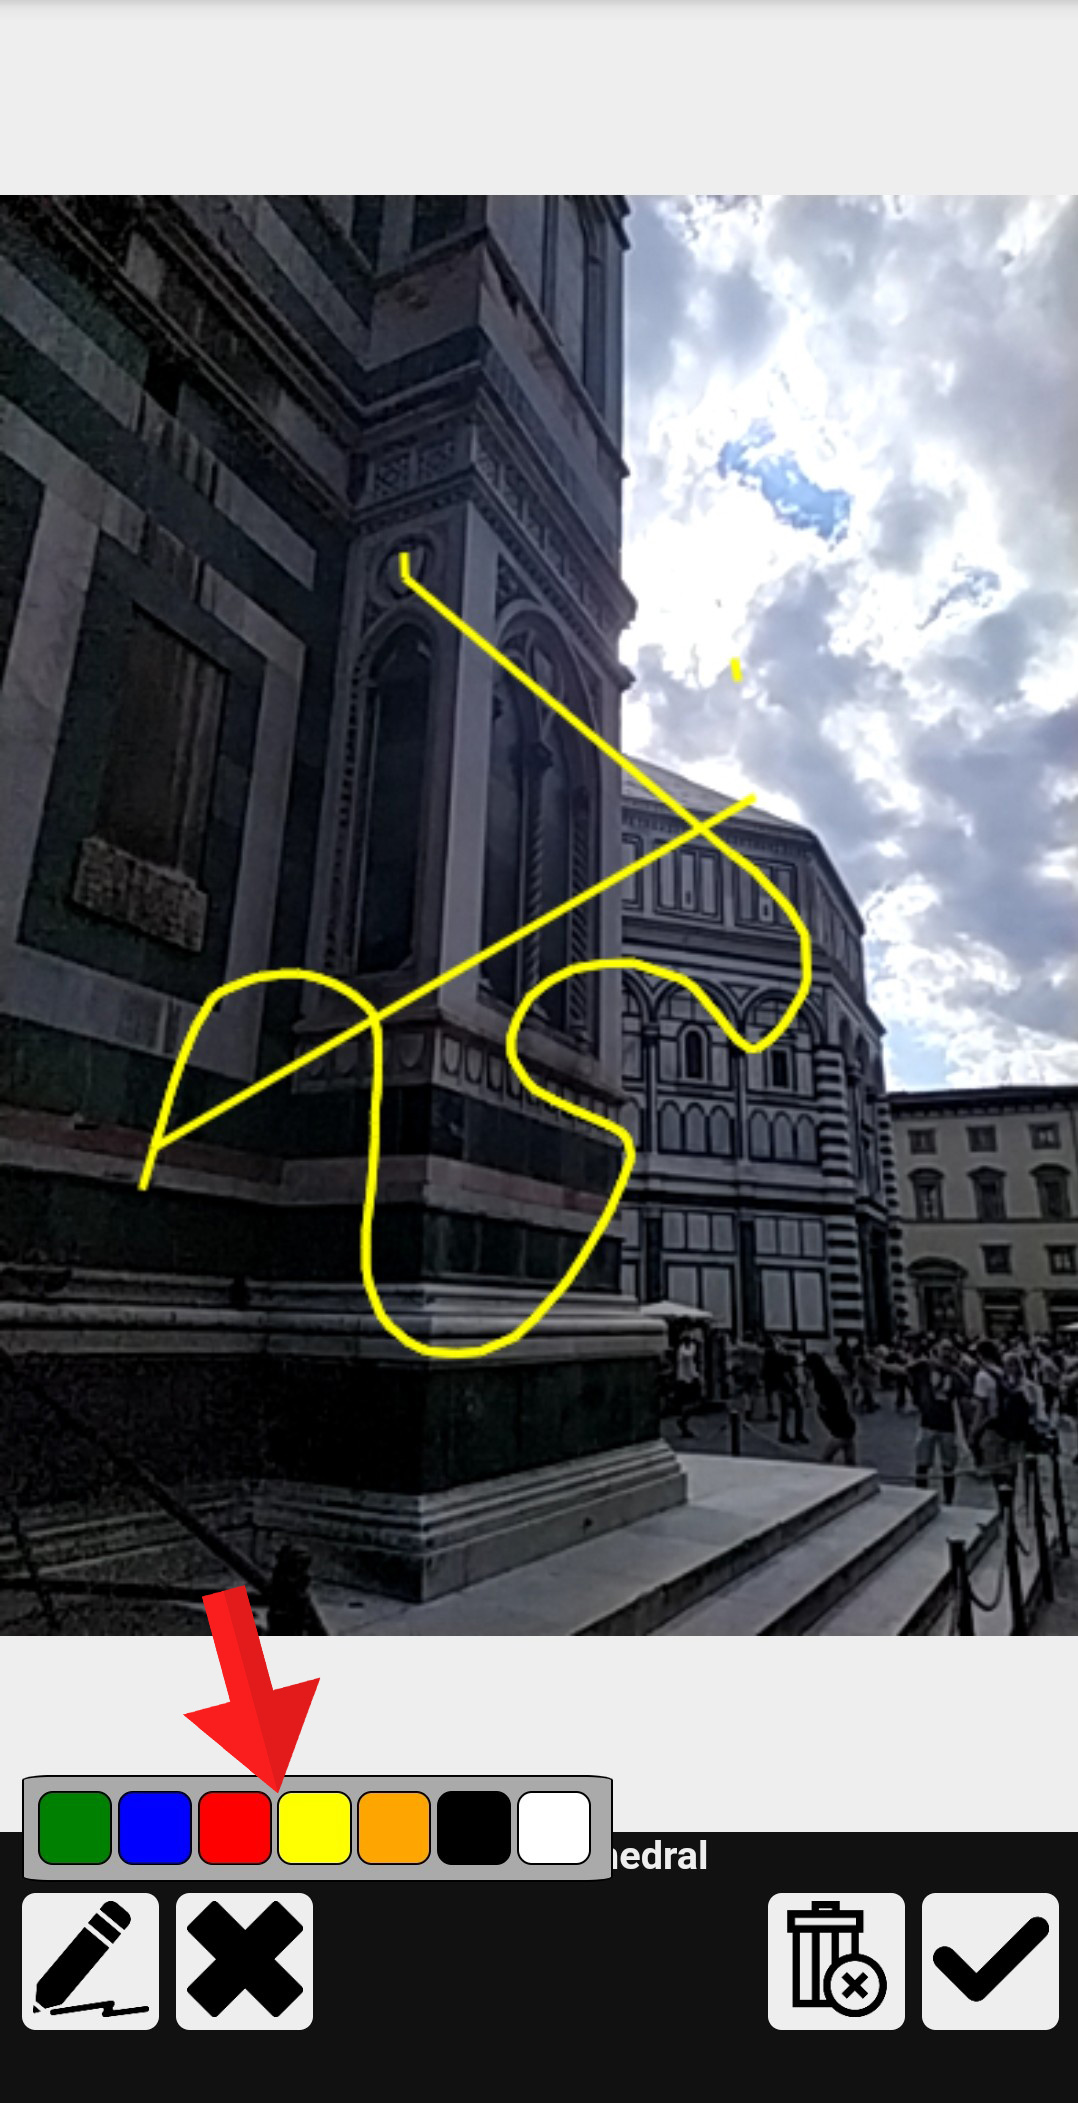
\includegraphics[scale=0.1]{"Immagini/editor1.jpg"}
 		\end{figure}
 	\item[] <5|only@5> 
		\begin{figure}[!h]
 			\centering
 			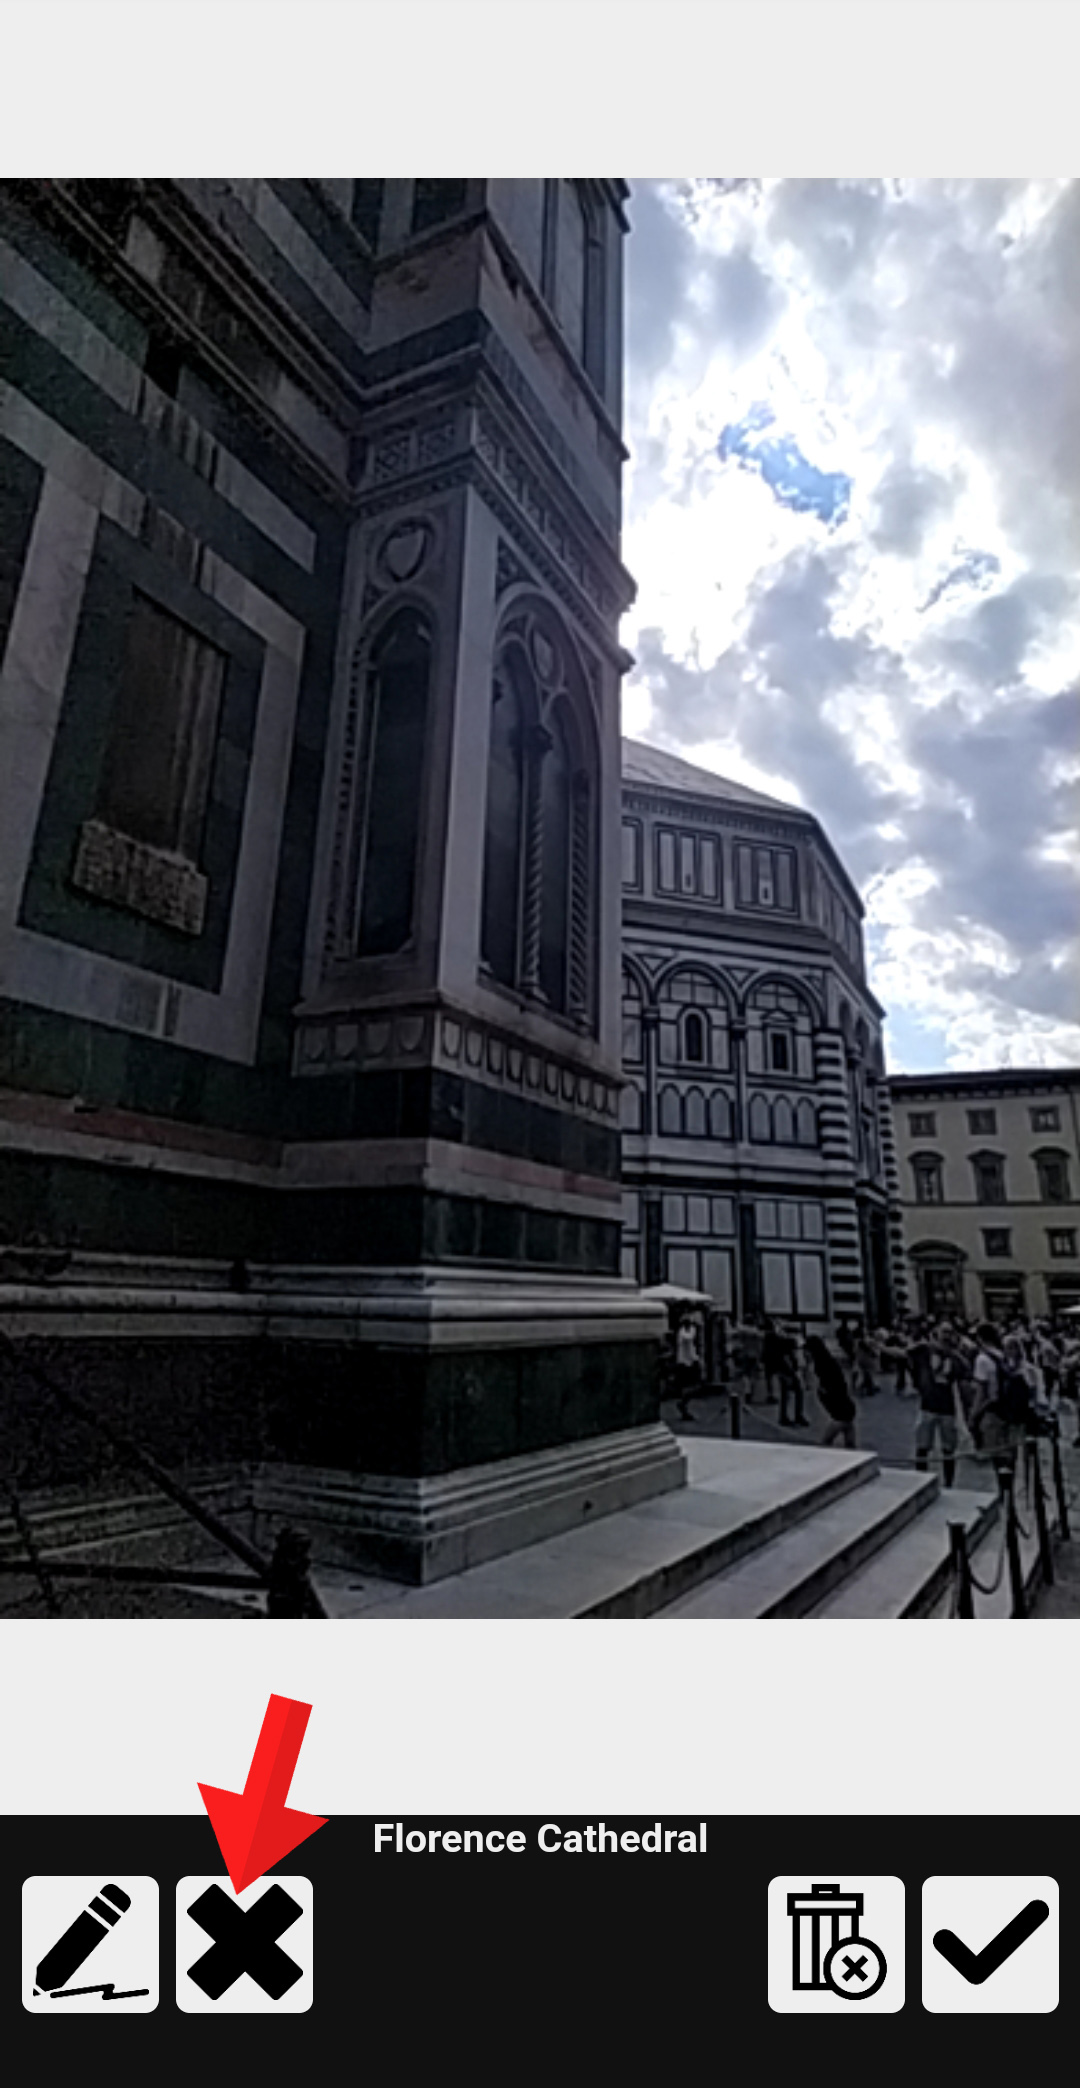
\includegraphics[scale=0.1]{"Immagini/editor3.jpg"}
 		\end{figure}
 	\item[] <6|only@6> 
		\begin{figure}[!h]
 			\centering
 			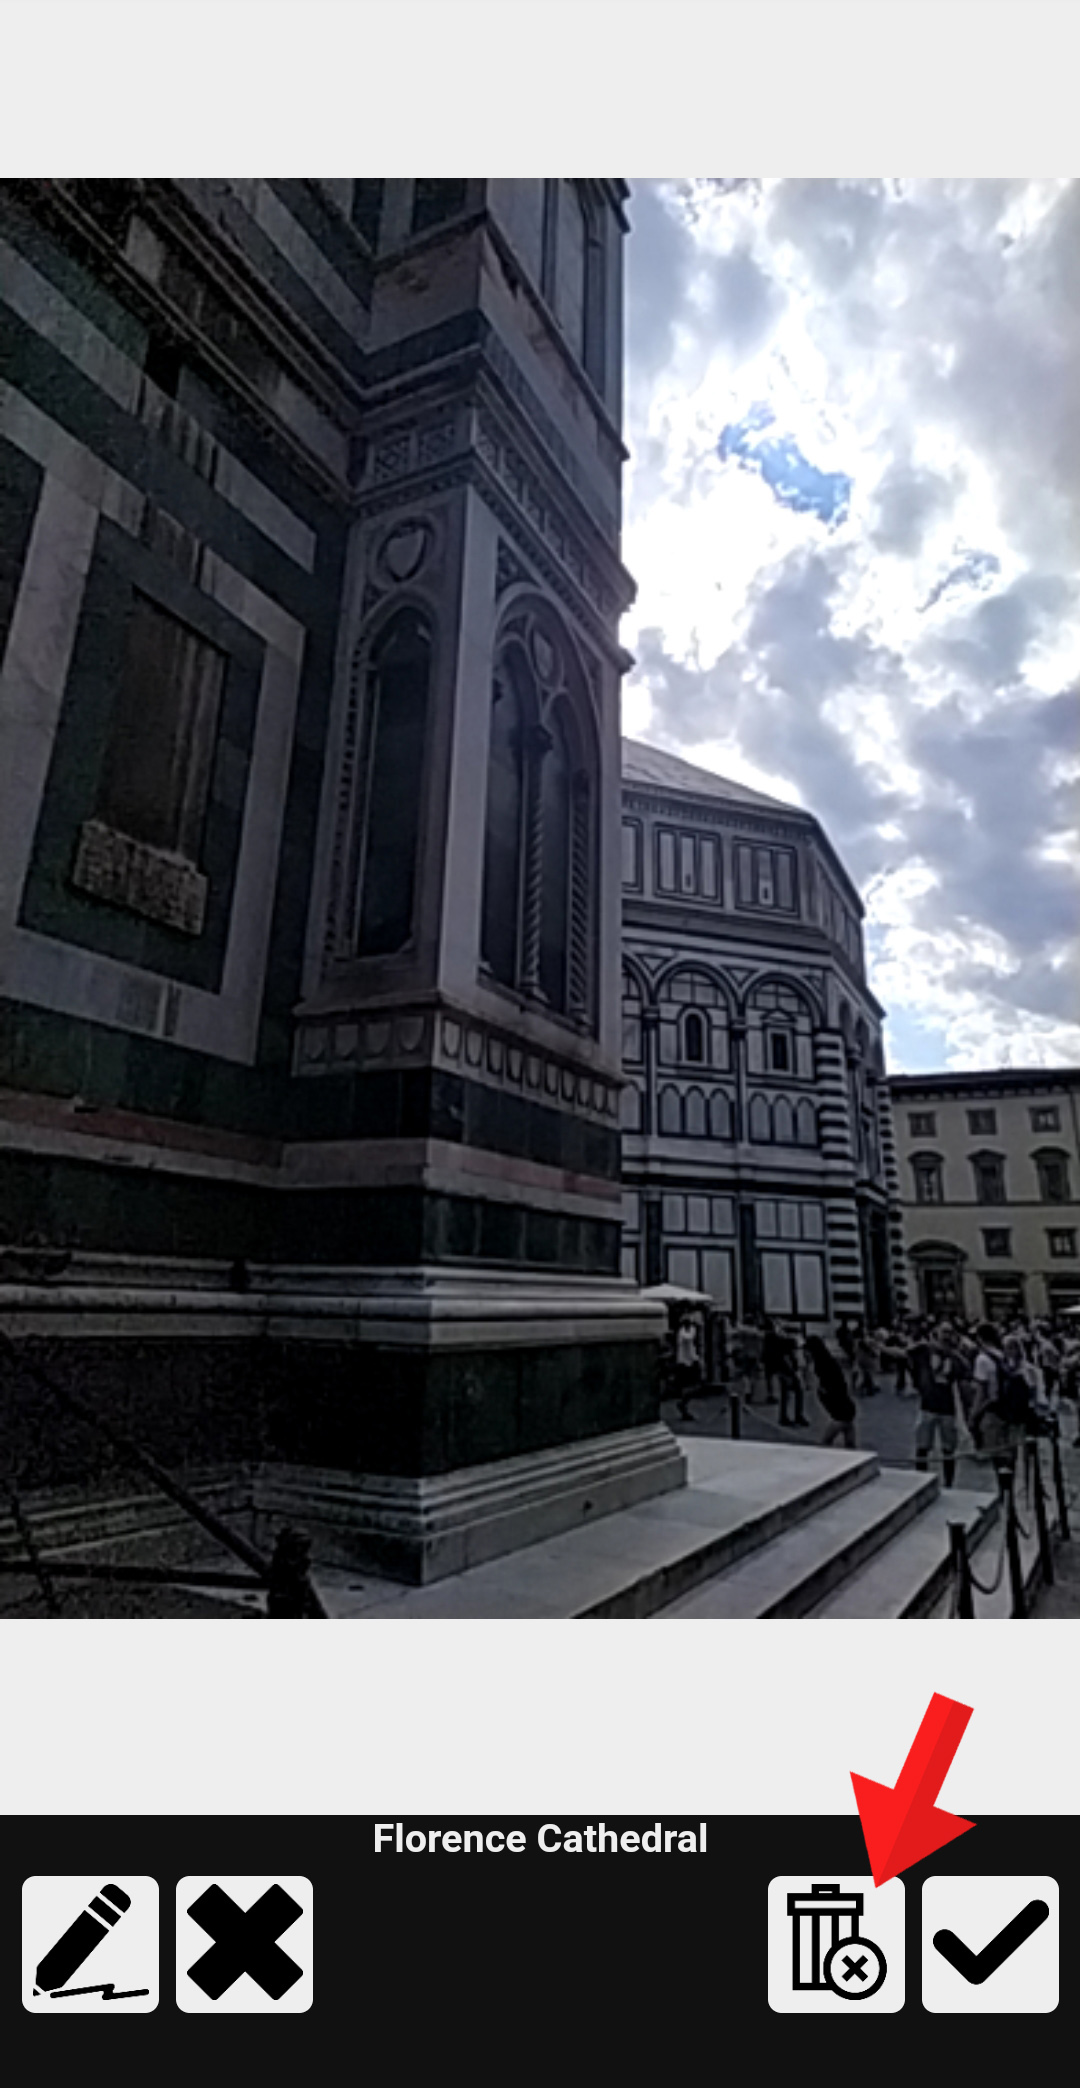
\includegraphics[scale=0.1]{"Immagini/editor6.jpg"}
 		\end{figure}
 	\item[] <7|only@7> 
		\begin{figure}[!h]
 			\centering
 			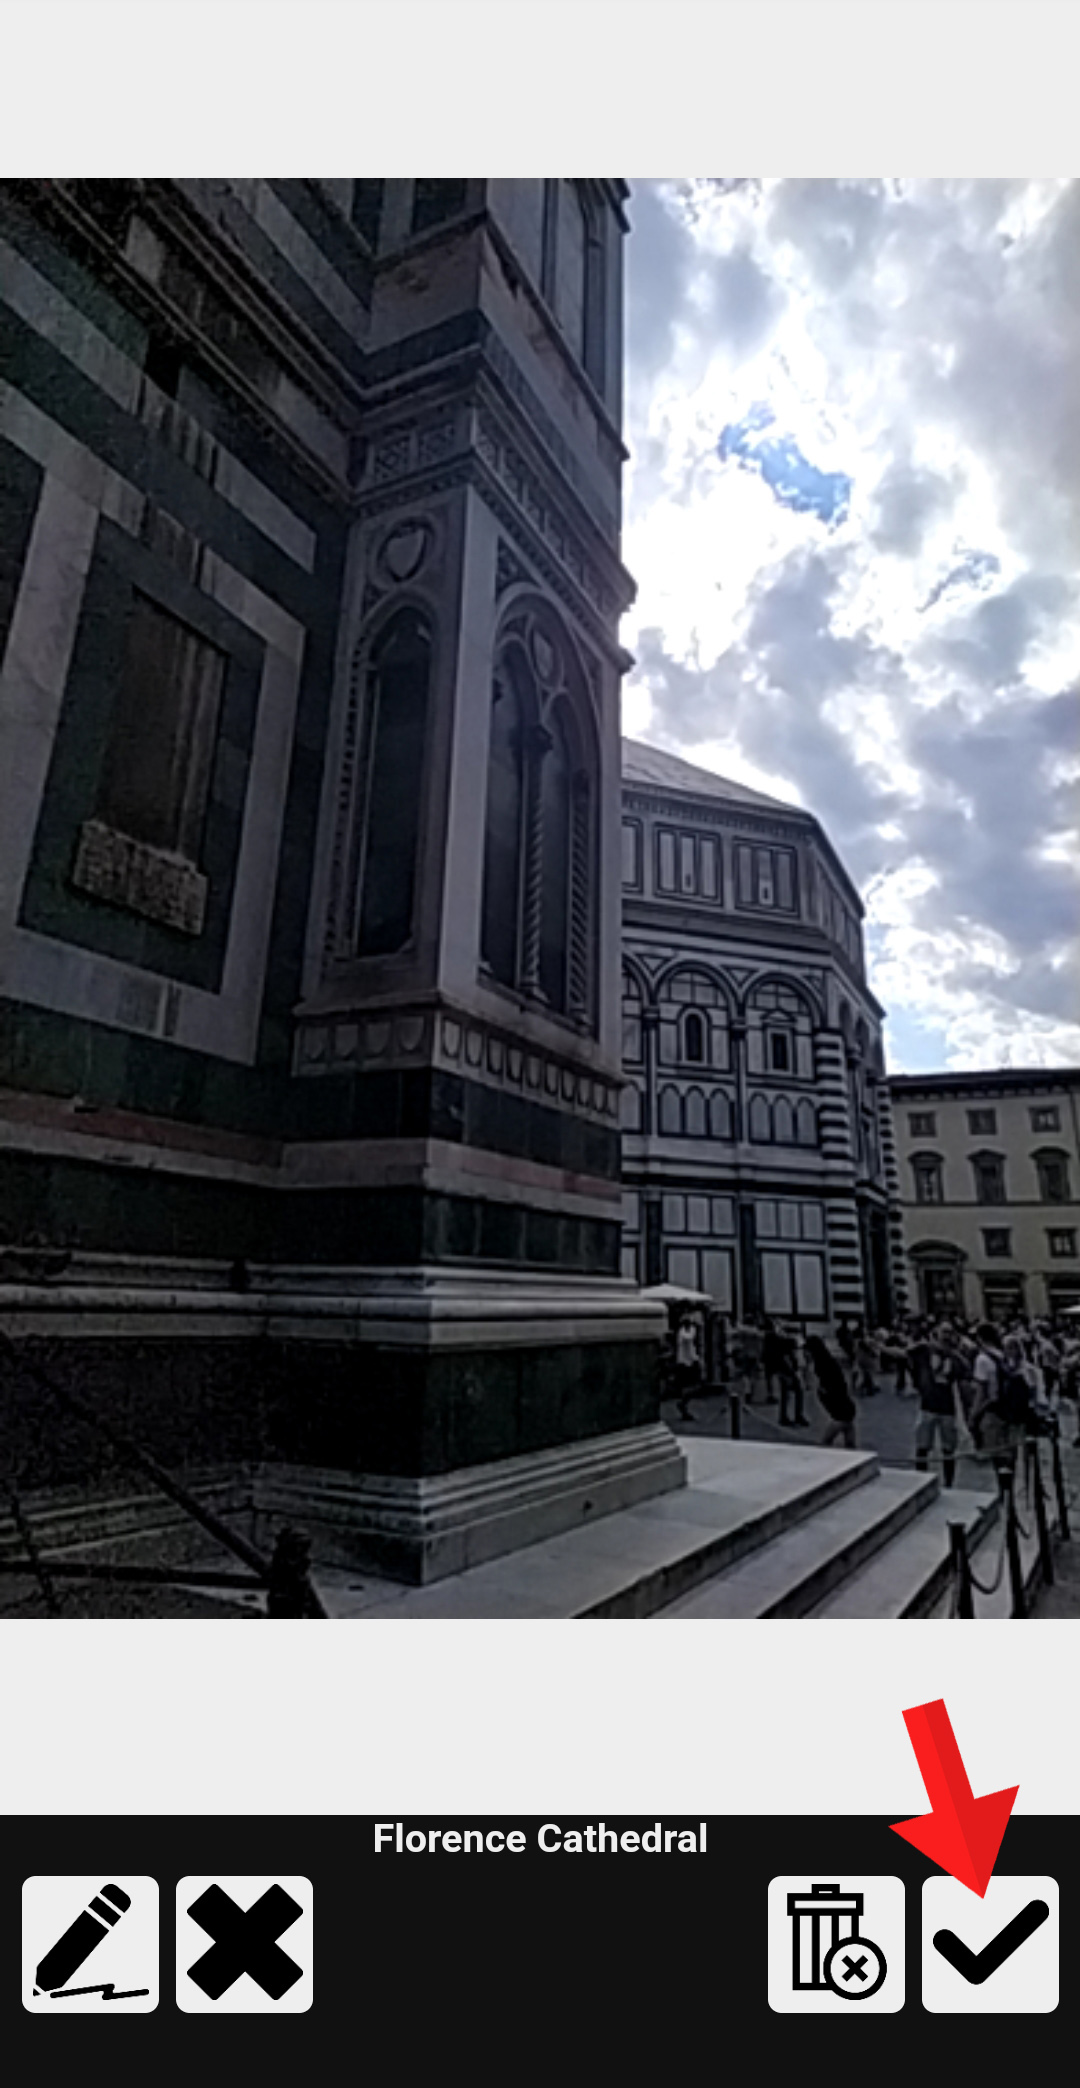
\includegraphics[scale=0.1]{"Immagini/editor5.jpg"}
 		\end{figure}
\end{itemize}
\end{columns}
\end{frame}

\begin{frame}
\frametitle{Galleria}
\begin{columns}
\column{0.5\textwidth}
\begin{itemize}
 	\item <2-> Nome del POI associato alla galleria
 	\item <3-> Pulsante tornare alla mappa e chiudere la galleria
 	\item <4-> Pulsanti per scorrere lo slider della galleria
 	\item <5-> Slider con foto singola 
 	\item <5-> \movie[externalviewer]{\color{blue} Esempio}{Video/galleria.mp4} 
\end{itemize}

\column{0.5\textwidth}
\begin{itemize}
	\item[] <1|only@1> 
		\begin{figure}[!h]
 			\centering
 			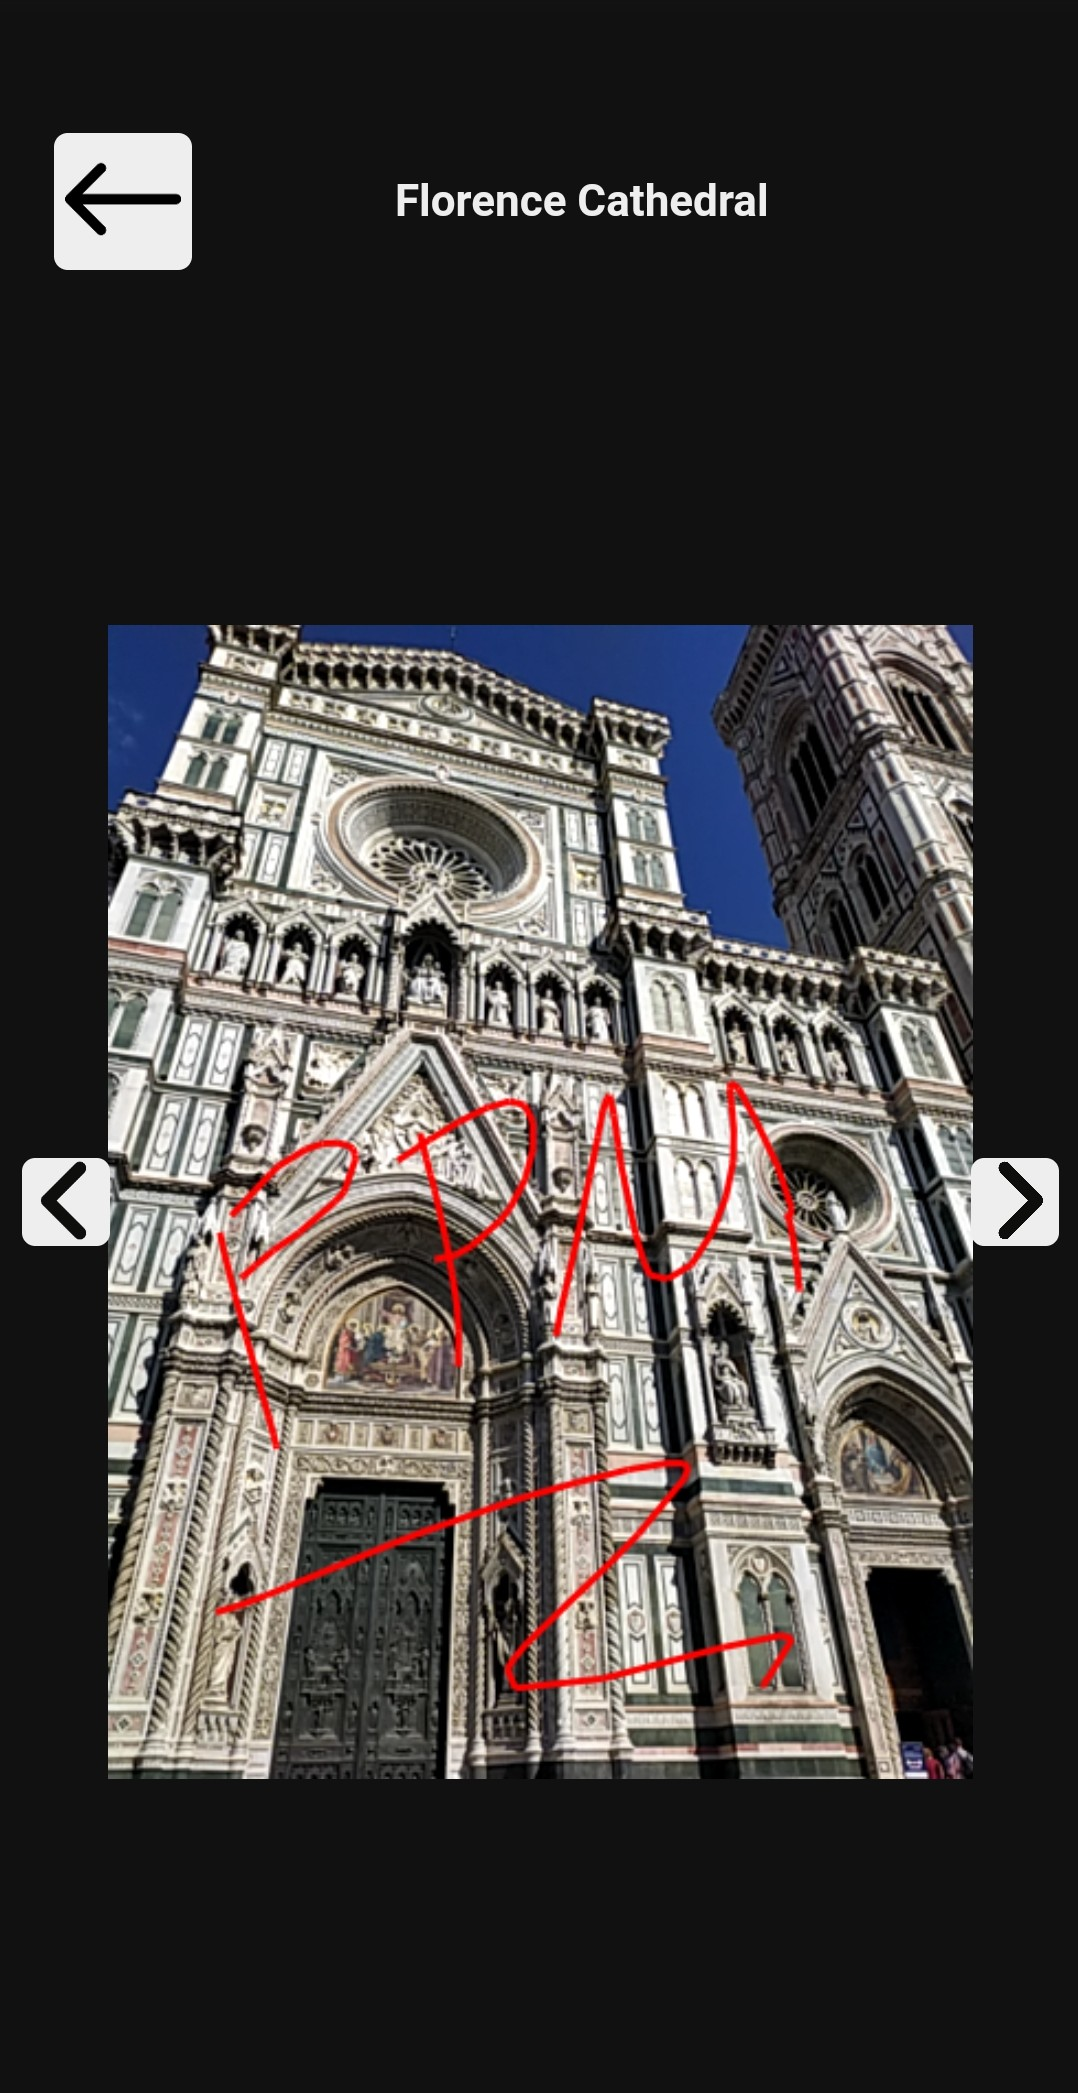
\includegraphics[scale=0.1]{"Immagini/slider_doppia.jpg"}
 		\end{figure}
 	\item[] <2|only@2> 
		\begin{figure}[!h]
 			\centering
 			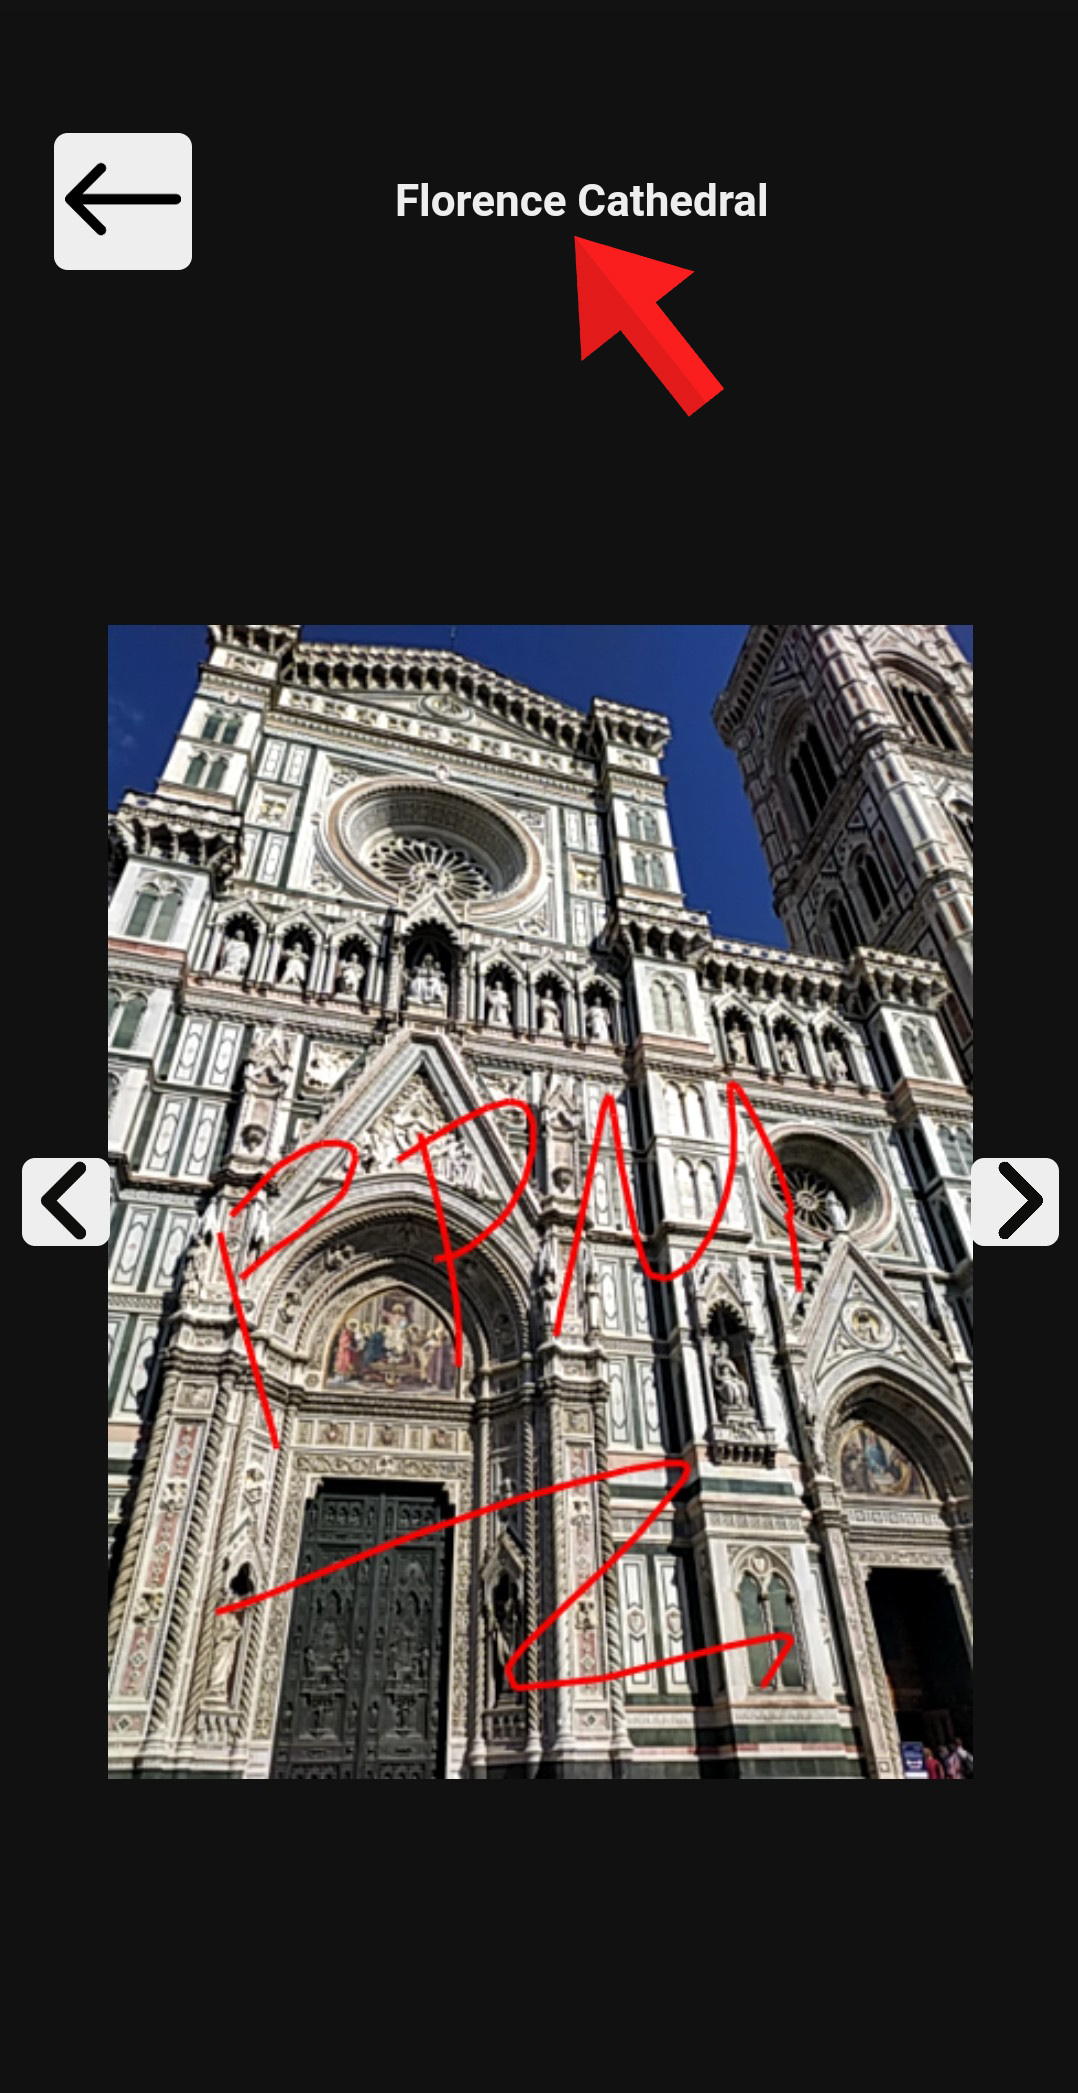
\includegraphics[scale=0.1]{"Immagini/slider_doppia2.jpg"}
 		\end{figure}
 	\item[] <3|only@3> 
		\begin{figure}[!h]
 			\centering
 			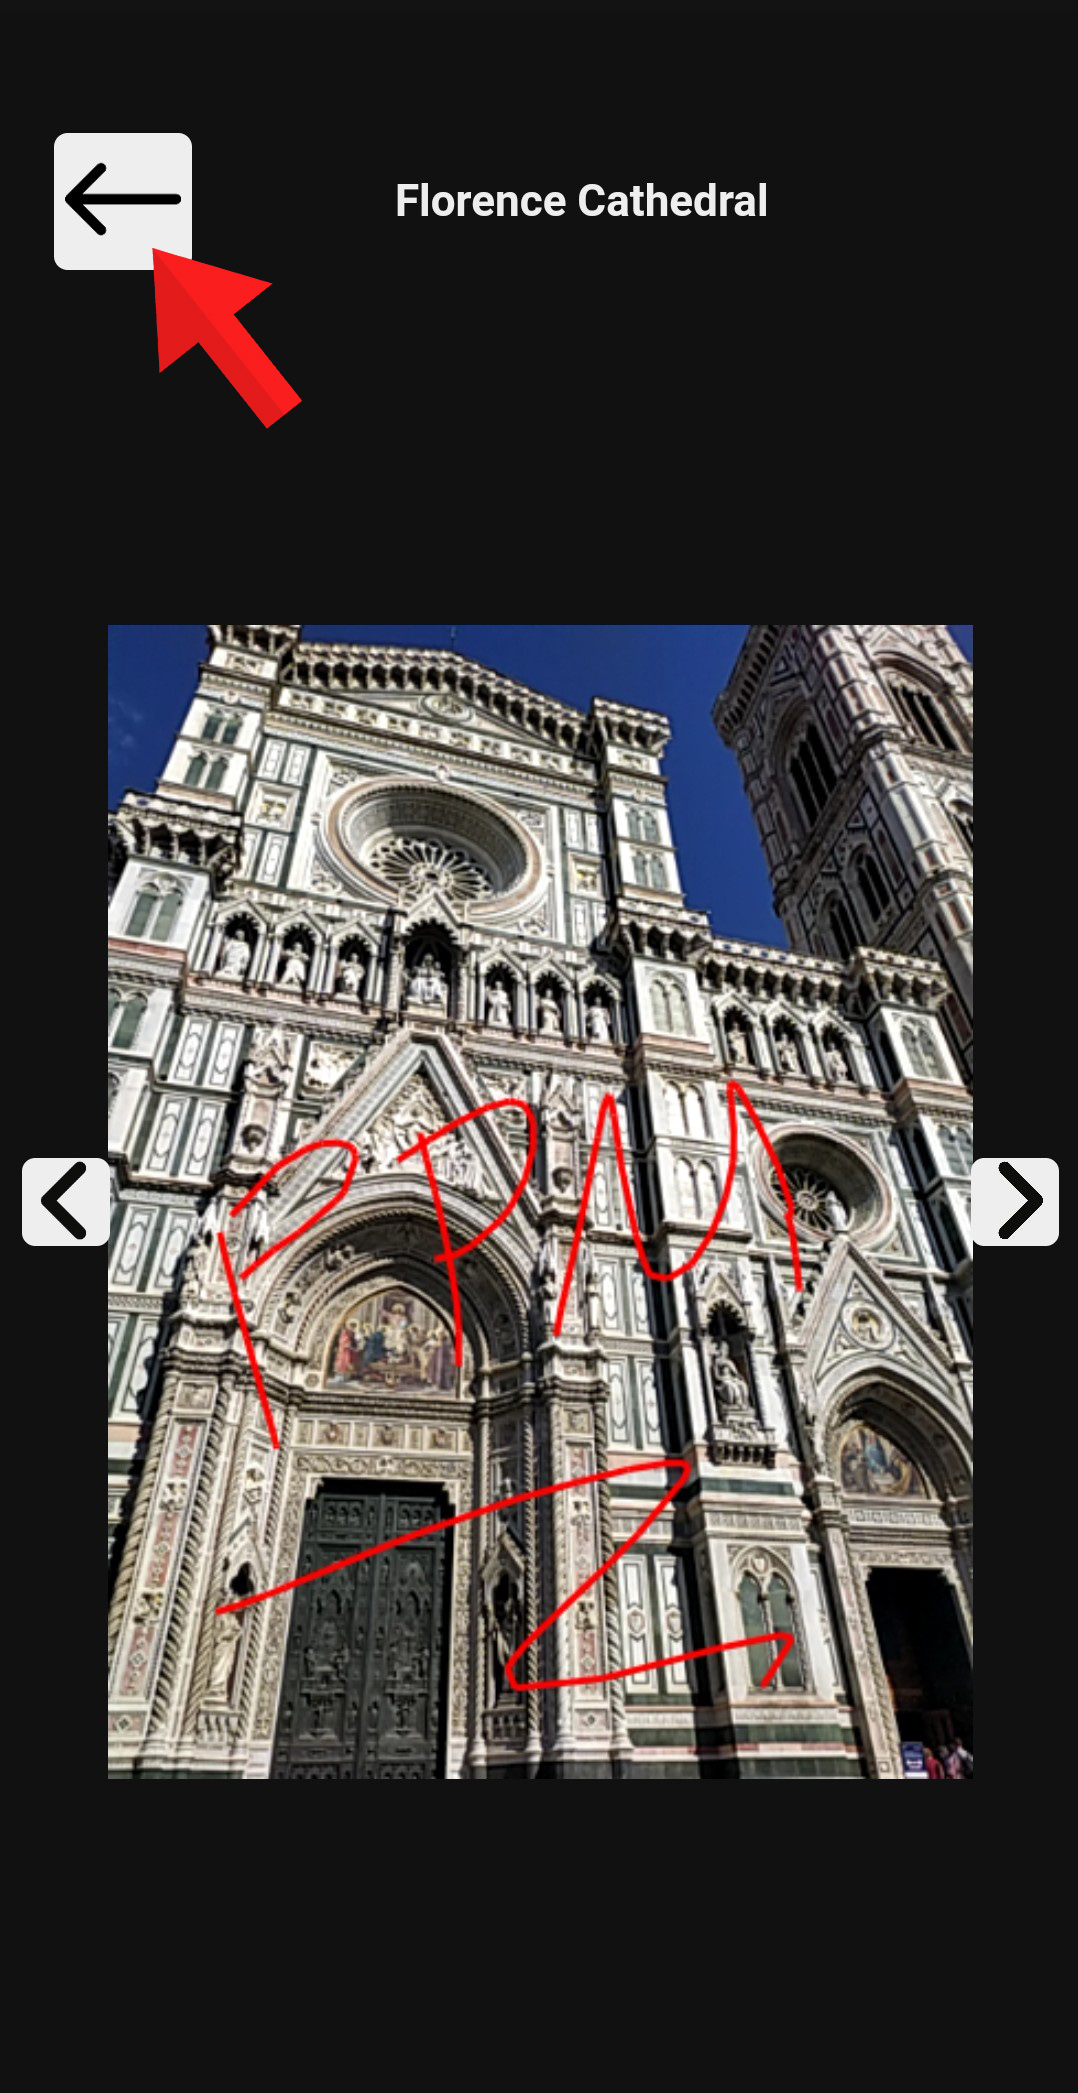
\includegraphics[scale=0.1]{"Immagini/slider_doppia1.jpg"}
 		\end{figure}
 	\item[] <4|only@4> 
		\begin{figure}[!h]
 			\centering
 			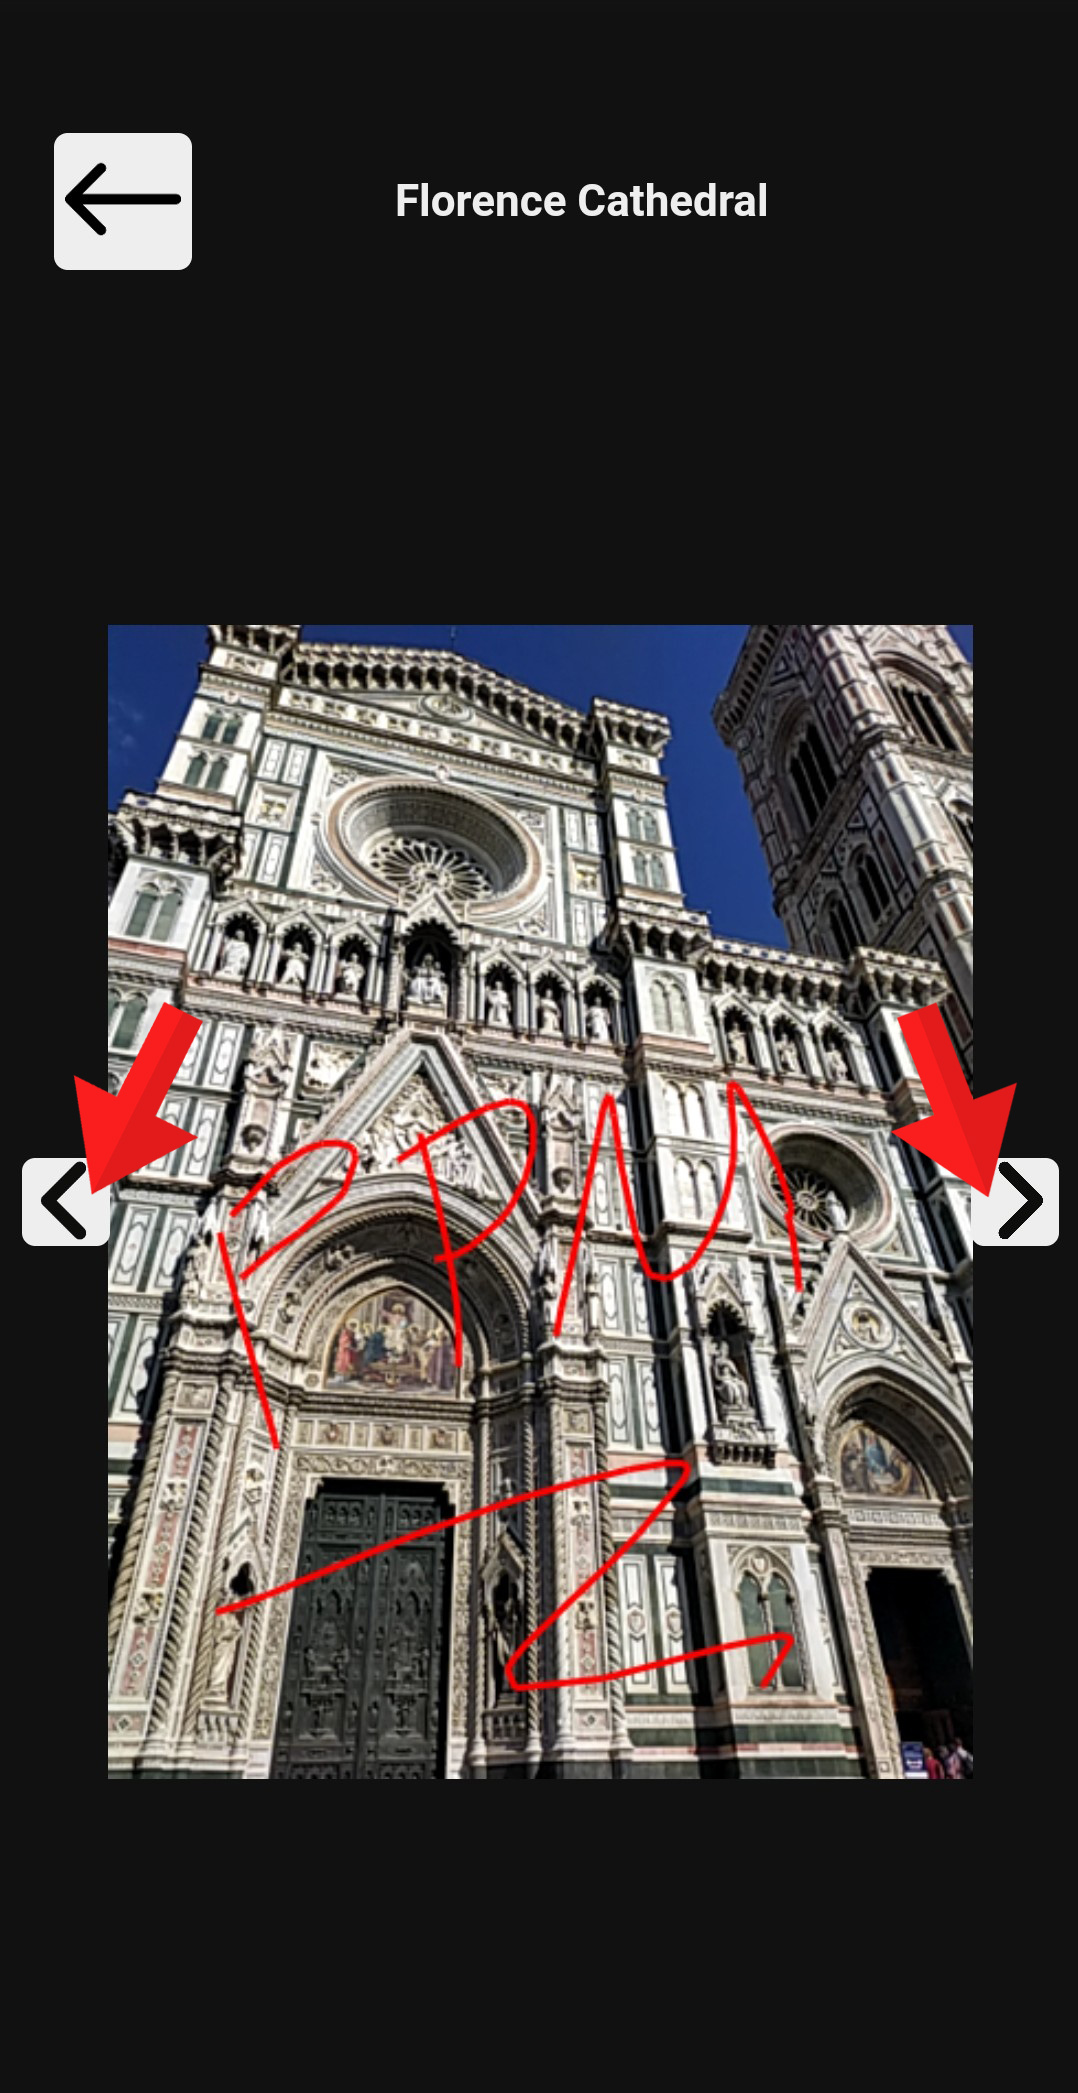
\includegraphics[scale=0.1]{"Immagini/slider_doppia3.jpg"}
 		\end{figure}
 	\item[] <5|only@5> 
		\begin{figure}[!h]
 			\centering
 			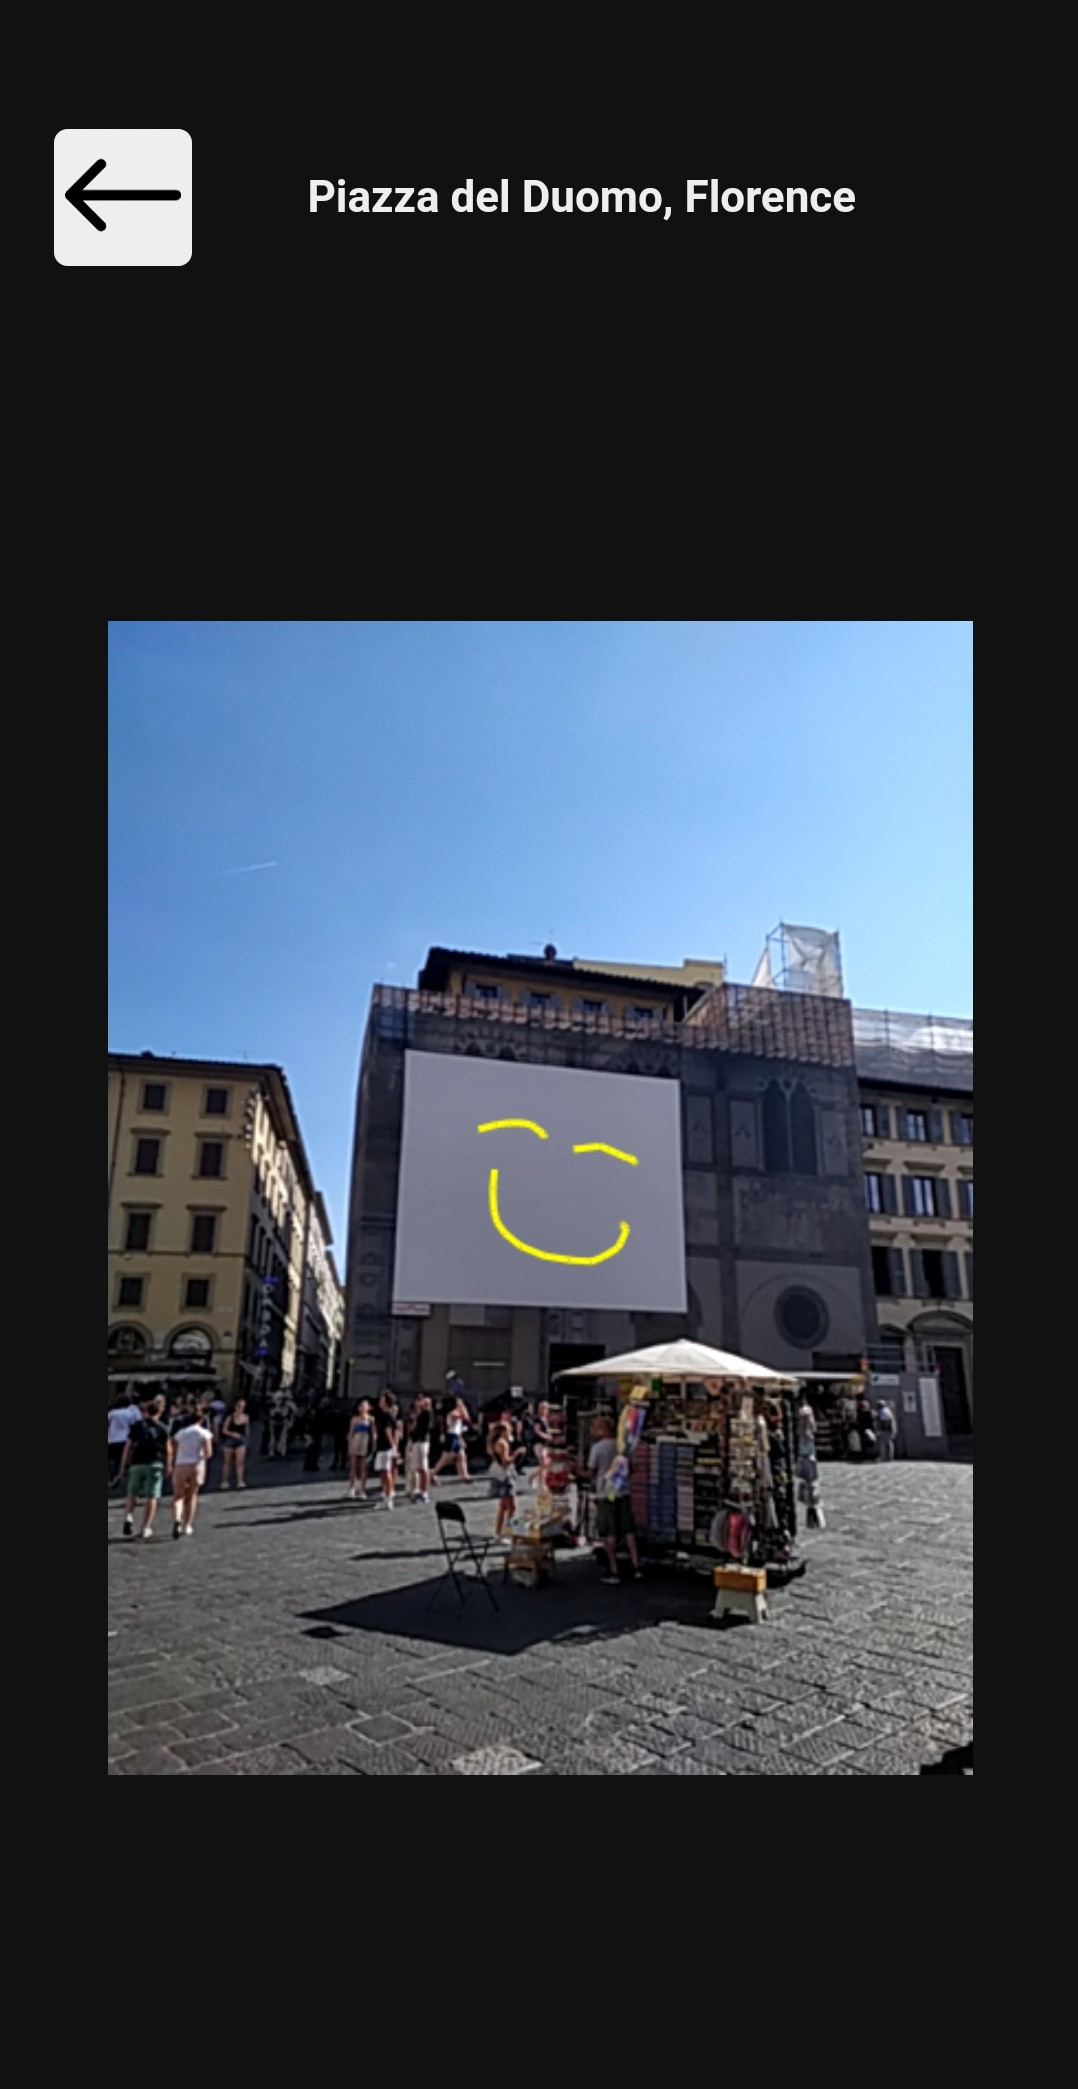
\includegraphics[scale=0.1]{"Immagini/slider_singola.jpg"}
 		\end{figure}
\end{itemize}
\end{columns}
\end{frame}

\begin{frame}
\frametitle{Test}
\begin{columns}
\column{0.4\textwidth}
\begin{itemize}
 	\item <1-> Test di speed eseguito sul sito \url{https://developers.google.com/speed/pagespeed/insights/} per versione Desktop e Mobile 
 	\item <3-> Test di Accessibility eseguito sul sito \url{https://wave.webaim.org/}
 	\item <3-> \url{https://snapandpost.altervista.org}
\end{itemize}

\column{0.6\textwidth}
\begin{itemize}
	\item[] <1|only@1> 
		\begin{figure}[!h]
 			\centering
 			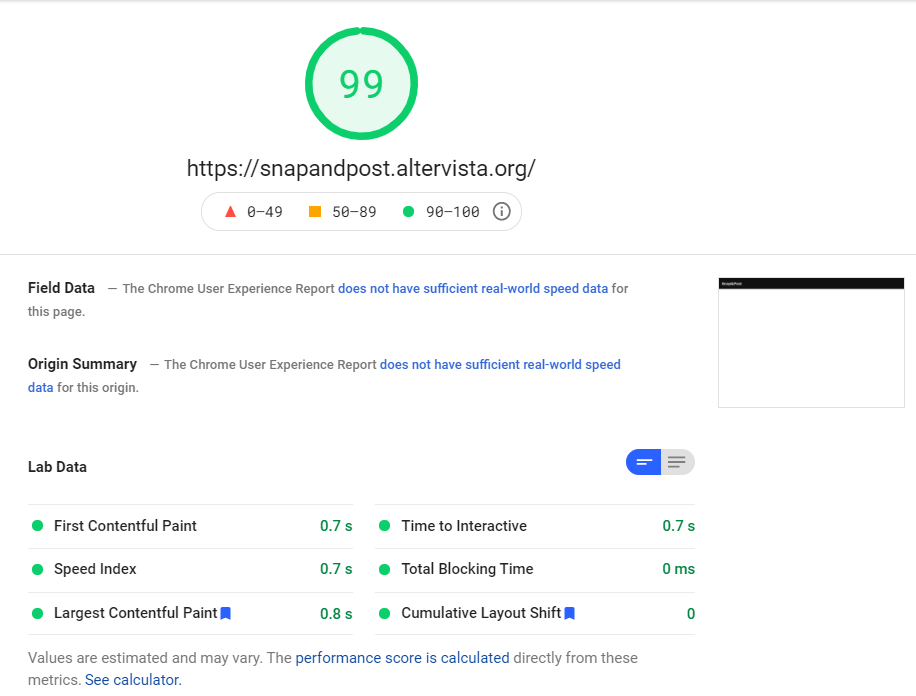
\includegraphics[scale=0.32]{"Immagini/speedDesktop.png"}
 		\end{figure}
 	\item[] <2|only@2> 
		\begin{figure}[!h]
 			\centering
 			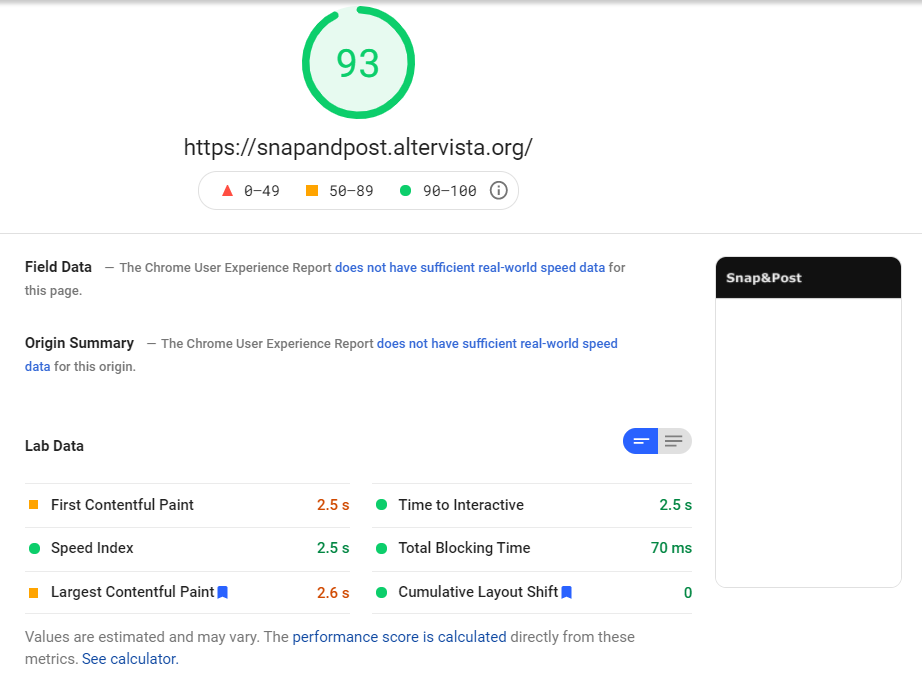
\includegraphics[scale=0.32]{"Immagini/speedMobile.png"}
 		\end{figure}
 	\item[] <3|only@3> 
		\begin{figure}[!h]
 			\centering
 			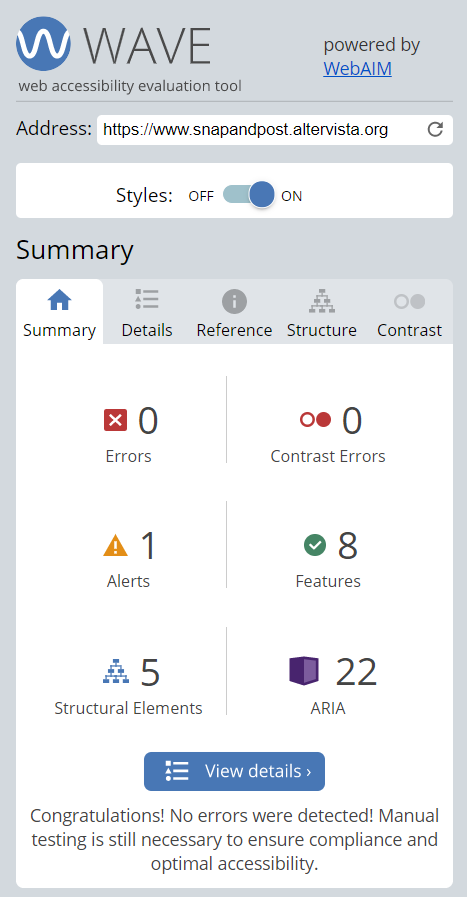
\includegraphics[scale=0.36]{"Immagini/accessibility.png"}
 		\end{figure}
\end{itemize}
\end{columns}
\end{frame}

\end{document}